\documentclass[11pt,a4paper,pdftex,parskip]{scrreprt}
\usepackage[ngerman]{babel}
\usepackage[utf8]{inputenc}
\usepackage[T1]{fontenc}
\usepackage[german]{fancyref}
\usepackage{scrhack,ngerman,listings,verbatim,graphicx,float,url,eurosym,textcomp} %german
\usepackage{amsmath,amsthm,amssymb,amsfonts,mathtools} %Mathematik

\usepackage[babel,german=swiss]{csquotes} %Anführungszeichen
\usepackage{cite,bibgerm,moreverb} %Litertur
\bibliographystyle{gerapali}
\usepackage[german]{nomencl} %Abkürzungsverzeichniss
%\usepackage[toc]{glossaries} %Glossar

\renewcommand{\nomname}{Abkürzungsverzeichnis}
\setlength{\nomlabelwidth}{0.2\hsize} % Punkte zw. Abkürzung und Erklärung
\renewcommand{\nomlabel}[1]{#1 \dotfill}
\makenomenclature
%\makeglossaries

\usepackage[left=40mm,right=20mm,top=30mm,bottom=30mm,headsep=10mm,includeheadfoot]{geometry}
\usepackage{scrpage2,setspace}
\pagestyle{scrheadings}
\automark[chapter]{chapter}
\onehalfspacing

\bibliographystyle{plain}

\begin{document}
	\clearscrheadfoot
	\ohead[\pagemark]{\pagemark}
	\begin{titlepage}
\vspace{4cm}
\begin{center}
Hochschule für Technik, Wirtschaft und Kultur\\
Fakultät Informatik, Mathematik und Naturwissenschaften 
\vspace{5cm}

\huge{\textbf{Belegarbeit}}\\
\normalsize
\vspace{1cm}
Ermittlung der Eignung und Einbettung \\von Sensoren zur Umwelterfassung in \\das Stadtlichtprojekt Leipzig
\\
\vspace{\fill}
\end{center}

\begin{flushleft}
\begin{tabular}{p{0.4\textwidth} p{0.5\textwidth}}
 \textbf{Autor:} & Robert Kupferschmied B. Sc.  \\ 
 & \\
 \textbf{Ko - Autor:} & Roy Meissner B. Sc.  \\
 & \\
 \textbf{Studiengang:} & Informatik, Master \\ 
 & \\
 \textbf{Studienfach:} & Mikrocontroller-Anwendungen \\ 
 & \\
 \textbf{Betreuende Personen:} & Prof. Dr. Klaus Bastian \\
 & Dipl.-Ing. Oliver Fasterding \\
 & Dipl.-Inf. (FH) Alexander Zahn \\
\end{tabular} 
\end{flushleft}

\end{titlepage}

	%
\begin{titlepage}
\begin{center}
\huge{\textbf{Lizenzhinweis}}
\end{center}
\vspace{4.5cm}

Die vorliegende Arbeit steht unter der Lizenz:
\vspace*{1cm}\\General Public License v3\vspace*{1cm}\\
Die Weitergabe des Inhaltes der Arbeit und eventuell beiliegender Zeichnungen und Daten im Gesamten oder in Teilen ist grundsätzlich erlaubt und erwünscht. Abschriften und Erweiterungen bezüglich des vorliegenden Arbeit sind ebenfalls erwünscht.

\begin{flushleft}
\vspace{\fill}
\today 
\end{flushleft}
\end{titlepage}
	%\include{Glossar}
	\pagenumbering{Roman}
	\tableofcontents
	\newpage

	\pagenumbering{arabic}
	\ihead{\rightmark}\chead{}\ohead[\pagemark]{\pagemark}
	\setheadsepline{0.2pt}
	\chapter{Einleitung}
	\section{Motivation}
		Beim Stadtlichtprojekt Leipzig geht es darum, die bereits seit langer Zeit bestehenden Natriumdampflampen der Stadtbeleuchtung gegen neuartige LED-Beleuchtungsmodule auszutauschen. Diese Module bieten im Vergleich zu den herkömmlichen Lampen viele Möglichkeiten die Lichtverteilung, die Lichtintensität, als auch die Lichtfarbe zu ändern. 
		
		Sinnvoll ist dies vor allem dann, wenn die Umgebungssituation ein spezielles Beleuchtungsprofil erfordert. Beispielsweise macht bei Regen eine andere Beleuchtung Sinn\footnote{Beispielsweise um Spiegelungen zu minimieren}, als dies bei trockener Straßenoberfläche der Fall wäre. Das verbessert wiederum die Sichtverhältnisse der Straßenteilnehmer und erhöht einhergehend die Sicherheit auf den Straßen. Vor allem in Blick auf die jährlichen Unfallraten im Straßenverkehr ist dies als sehr sinnvoll zu erachten.
		
		Um die dafür nötigen Umgebungsverhältnisse aufzunehmen, muss letztlich eine Sensorik eingesetzt werden. Diese wird an und in der Umgebung der Lampenköpfe installiert, welche über die Stadt verteilt werden und sollte zuverlässig Verhältnisse wie Regen, Nebel oder Oberflächeneisbildung erkennen können.
		\newpage
	\section{Ausgangslage}
		Es existiert bereits ein Prototyp der Lampenköpfe, welcher eine Steuereinheit enthält. Diese besteht aus einem speziellen Mikrocontroller samt einer Vorschaltung für die Netzwerkfähigkeit, einem Modul das die LED Streifen ansteuern kann sowie einem Temperatursensor, der direkt auf dem Board angebracht ist.
	\section{Ziel der Arbeit}
		Das Ziel der Arbeit besteht darin, verschiedene Sensoren zur Umwelterfassung zu bewerten und eine Referenzimplementierung auf der Plattform mbed NXP LPC1768 bereitzustellen.
		
		Dazu wurden drei Sensoren, zwei Temperatur- und Feuchtigkeitssensoren, ein Regensensor und ein Empfangsmodul für das allgemein ausgestrahlte Zeitsignal DCF77 bereitgestellt. Deren Funktionalität muss auf der Plattform unter Beachtung des Ressourcenverbrauchs implementiert und getestet werden.
		
		Letztlich soll die Sensorik noch exemplarisch vermessen und dokumentiert werden.
	\chapter{Fachliches Umfeld / Technische Grundlagen}
	\section{I$^{2}$C}
		\nomenclature{I²C}{Inter-Integrated Circuit}
		I$^{2}$C steht für Inter-Integrated Circuit. Es handelt sich hierbei um ein von Philips Semiconductors\footnote{Heute: NXP Semiconductors} entwickelten seriellen Datenbus. Ursprünglich konnten mit diesem Bus Datenübertragungsraten von 100 kbit/s erreicht werden. Mit dem aktuellen Standard\footnote{Version 3.0} von 2007 erreicht man Datenraten von bis zu 3,4 Mbit/s. 
		
		I$^{2}$C zeichnet sich dadurch aus, dass der Bus nur ein Leitungspaar benötigt. Trotz dieses vergleichsweise einfachen Aufbaus ist I$^{2}$C sehr flexibel.
		\subsubsection{Vorteile von I$^{2}$C:}
			\begin{enumerate}
				\item Nur zwei Busleitungen benötigt
				\item Keine Harten Baud-Raten-Anforderungen
				\item Einfache Master-Slave Beziehung der Buskomponenten
				\item Jede Komponente hat eine eindeutige Adresse
				\item Echter Multimasterbus mit Kollisionsbehandlung
			\end{enumerate}
			
			\cite{I2C}
		\subsection{Adressierung}
			Üblicherweise benutzt I$^{2}$C 7-Bit Adressen. Durch diese stehen 128 möglich Adressen zur Verfügung. Es existieren jedoch 16 reservierte Adressen, weswegen nur 112 Adressen vergeben werden können. In neueren Standards\footnote{ab Version 1.0} werden 10 Bit zur Adressierung verwendet, wodurch bis zu 1008 Geräte adressiert werden können.
			
			Zu erwähnen ist, dass bei I$^{2}$C immer 8 Bit Blöcke gesendet werden. Das letzte Bit der Adressierung wird dazu genutzt, dem Gerät mitzuteilen ob es sich um ein Lese-(1) oder eine Schreiboperation(0) handelt.
			
			\cite{I2C}
	\section{Elektrolytische Wechselspannungsmessung}
		Die elektrolytische Wechselspannungsmessung wird benutzt um die Leitfähigkeit, beziehungsweise die Impedanz eines bestimmtem Elektrolyts feststellen zu können.
		
		Typischerweise wird zur Widerstandsmessung eine Gleichspannung verwendet. Da bei einem Elektrolyt die Gleichspannung jedoch eine Debye-Schicht erzeugen würde, wird zur Widerstandsmessung von Elektrolyten eine Wechselspannung verwendet, welche diese Schicht nicht erzeugt. Mittels der Wechselspannung kann die Impedanz \underline{Z} und der Scheinwiederstand Z des Elektrolyts über die Formeln
		\[ \underline{Z} = \frac{u(t)}{i(t)}\hspace{1cm}Z = \frac{\hat{u}}{\hat{i}} \]
		berechnet werden. Der Kehrwert des Widerstands normiert auf ein dimensioniertes Stück des leitenden Materials gibt letztlich die Leitfähigkeit des Elektrolyts an.
		
		\cite{Impedanz}, \cite{Leitwert}
	\section{Mercurial}
		\nomenclature{VCS}{Versionsverwaltungssystem (Version Control System)}
		Mercurial ist ein verteiltes Versionsverwaltungssystem (VCS). Es wurde zeitgleich mit dem VCS Git entwickelt und war anfangs als VCS für den Linux Kernel gedacht. Für diesen wurde jedoch zeitnah das von Linus Torvalds entwickelte Git eingesetzt. Daher musste sich Mercurial zu einem eigenständigem VCS weiterentwickeln.
		
		Mercurial setzt sonst auf den gleichen Spezifikationen wie Git auf, wird aber oft als das einfachere System bezeichnet. Es bietet verteilte Versionskontrolle, Geschwindigkeit, Unterstützung durch große Hosting-Plattformen und Datensicherheit.
		
		\cite{Mercurial}
	\chapter{Evaluierung}
	Welche Software und welche speziellen Hardwaremodule bezüglich des Projekts benutzt werden sollten wurde im Voraus festgelegt und an dieser Stelle entsprechend der Auswahl vorgestellt.
	\section{Software}
		\subsection{Entwicklungsumgebung}
			Bezüglich des Mikrocontrollers \enquote{mbed NXP LPC1768} wird vom mbed-Projekt eine Online-Entwicklungsumgebung bereitgestellt, die im Projekt verwendet werden sollte.
			
			Die Entwicklungsumgebung bietet:
			
			\nomenclature{SDK}{Software Development Kit}
			\begin{itemize}
				\item High level C/C++ SDK
				\item Kochbuch mit publizierten Bibliotheken und Projekten
				\item Editer mit Code-Highlighting
				\item Projektbaumverwaltung
				\item Compiler
				\item Versionsverwaltung Mercurial
			\end{itemize}
			
			Weiterhin kann das Projekt aus der Entwicklungsumgebung sehr einfach in andere Umgebungen exportiert, beziehungsweise von diesen importiert werden. Zu diesen Umgebungen zählen unter anderem die \enquote{GCC ARM Embedded} und die \enquote{GCC Code Sourcery}.
			
			Zum Projekt selbst werden auf einer Übersichtsseite mehrere Fakten zusammengetragen. Diese enthalten unter anderem, ob die importierten Bibliotheken auf dem aktuellen Stand sind und wie die Speichernutzung auf der aktuellen Plattform aussieht.
		\subsection{Bibliotheken}
			Die vom mbed-Projekt und seinen Nutzern bereitgestellten Bibliotheken sind sehr umfangreich. Bereits die Standardbibliothek macht das arbeiten mit dem Controller sehr einfach und im Vergleich zu anderen Mikrocontrollern ist diese Bibliothek als sehr Benutzerfreundlich einzustufen.
			
			Die Standardbibliothek fasst alle Dinge zusammen, die am Controller selbst eingestellt werden können. Soll beispielsweise ein Pin als \enquote{Output-Pin} definiert werden, ist dies über diese Bibliothek möglich. Auch die höheren Funktionen, wie die I$^{2}$C Benutzung, stellt diese Bibliothek bereit.
			
			Zusätzlich zur Standardbibliothek wurde im Projekt die Bibliothek \enquote{RTOS} benutzt. Diese stellt eine Implementierung eines Echtzeit-Betriebssystems dar, das viele Dinge auf einem Mikrocontroller vereinfacht. Von der Bibliothek wird unter anderem bereitgestellt:
			
			\begin{itemize}
				\item Thread-Modell mit Scheduler
				\item Inter-Prozess-Kommunikation
				\item Semaphore
				\item Interrupt-Service-Routinen
				\item Signale
				\item Speicher-Pools
			\end{itemize}
			
			In der vorliegen Arbeit wurde dabei Gebrauch vom Thread-Modell, den Sempahoren und den Interrupt-Service-Routinen gemacht.
			
			\cite{RTOS}
	\section{Hardware}
		\subsection{Mikrocontroller \enquote{mbed NXP LPC1768}}
			Der Mikrocontroller wurde vom mbed-Projekt der Firma ARM Holdings plc bereitgestellt. Er ist dafür gedacht eine schnelle Prototypen-Entwicklung auf einer, für einen Mikrocontroller leistungsfähigen Plattform durchführen zu können.
			
			Der benutzte Mikrocontroller ist die größte Ausbaustufe der erhältlichen Prototyp-Module. In der folgenden \enquote{Feature-List} \cite{LPC1768} und der Abbild \ref{fig:LPC1768-pinout} ist kurz aufgeführt, was der Controller bereitstellt.
			
			\begin{itemize}
				\item High performance ARM® Cortex™-M3 Core
				\item 96MHz, 32KB RAM, 512KB FLASH
				\item Ethernet, USB Host/Device, 2xSPI, 2xI$^{2}$C, 3xUART, CAN, 6xPWM, 6xADC, GPIO
				\item 40-pin 0.1" pitch DIP package, 54x26mm
				\item 5V USB or 4.5-9V supply
				\item Built-in USB drag 'n' drop FLASH programmer
			\end{itemize}
			
			\begin{figure}[H]
				\centering
				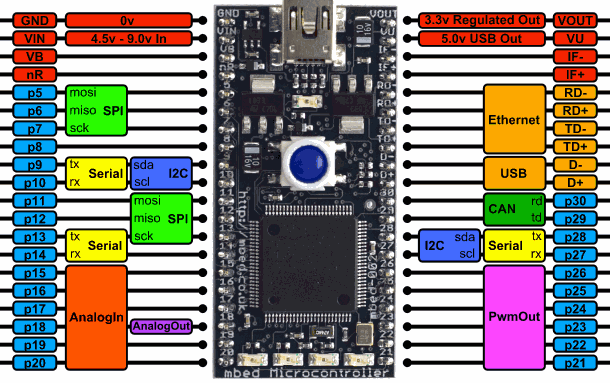
\includegraphics[width=0.7\linewidth]{Grafiken/LPC1768-pinout}
				\caption[mbed NXP LPC1768 Pinout]{mbed NXP LPC1768 Pinout\protect\footnotemark}
%				\caption[TI Beispiel zum Schedulerverhalten]{TI Beispiel zum Schedulerverhalten\protect\footnotemark}
				\label{fig:LPC1768-pinout}
			\end{figure}
			\footnotetext{Quelle: \cite{LPC1768}}
			
			\cite{LPC1768}
		\subsection{Empfangsmodul DCF77}
			Das im Projekt benutzte Empfangsmodul \enquote{C-Control DCF-Empfängerplatine} besteht aus einer fertigen Schaltung zum Empfang des DCF77-Signals. Verbaut ist eine Ferritkernantenne, welche an einer Schaltung befestigt ist, die das empfangene Signal auswertet und an zwei Ausgängen als Logikpegel entsprechend der Versorgungsspannung ausgibt. Da diese Ausgänge jedoch offene Kollektoren sind und nur mit 1 mA belastet werden können, muss gegebenenfalls eine Vorschaltung errichtet werden, die das Signal für einen Mikrocontroller aufwertet.
			
			\newpage
			Die technischen Daten des Empfängers sind:
			
			\begin{itemize}
			 \item Versorgungsspannung 2,5 bis 15 V DC
			 \item Stromaufnahme 3 mA
			 \item Ausgabe: Signal, Signal invertiert
			 \item Signalausgänge sind offene Kollektoren die maximal mit 30 V, 1 mA belastet werden können
			\end{itemize}
			
			\begin{figure}[H]
				\centering
				\includegraphics[width=0.6\linewidth,height = 8cm]{Grafiken/DCF77}
				\caption[DCF77 Antenne und Platine]{DCF77 Antenne und Platine\protect\footnotemark}
				\label{fig:DCF77}
			\end{figure}
			\footnotetext{Quelle: \cite{DCF77}}
			
			\cite{DCF77}, \cite{DCF77Manual}
		\subsection{Temperatur-/Feuchtigkeitssensor HYT2x1}
			\subsubsection{Daten zum HYT271/241}
				\begin{figure}[H]
				\centering
				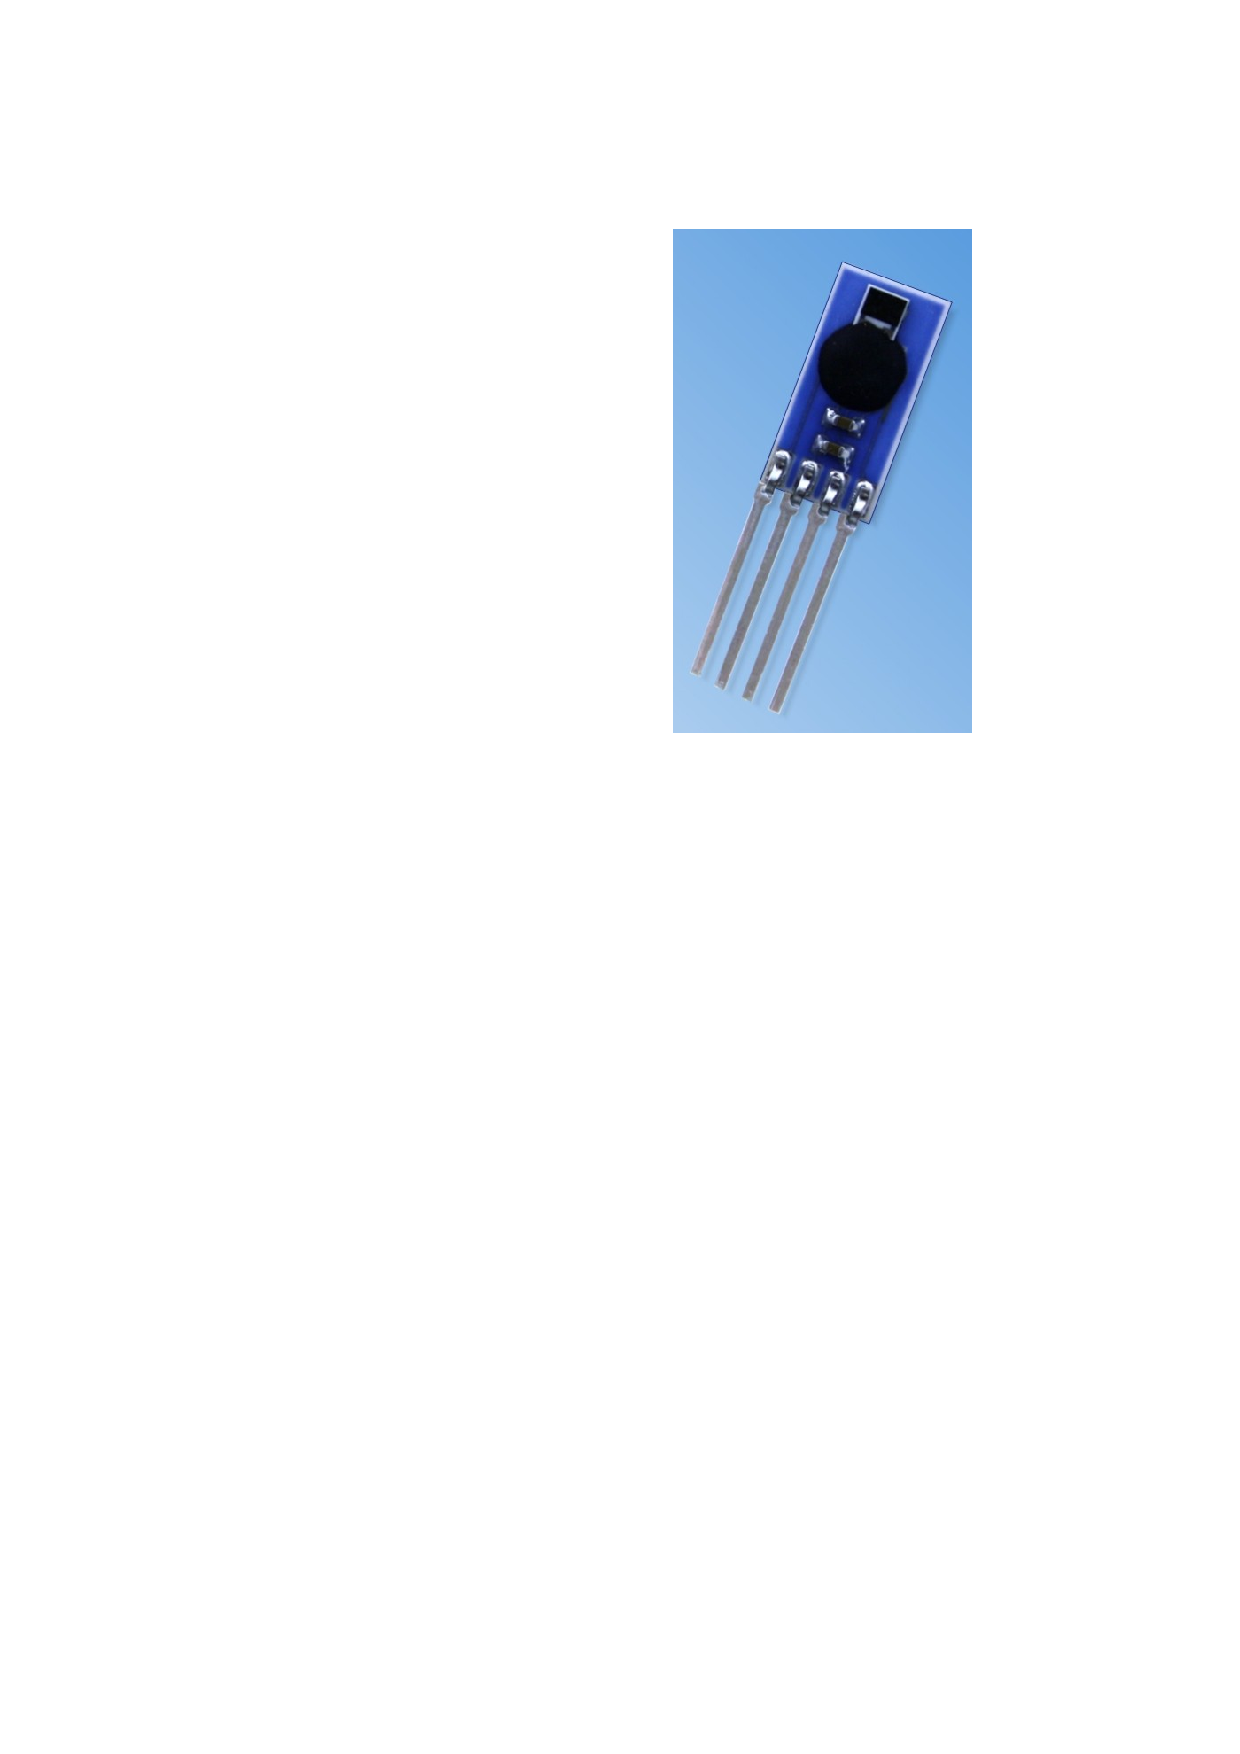
\includegraphics[height=5cm]{./Grafiken/HYT271}
				\caption[HYT271]{HYT271\protect\footnotemark}
				\label{fig:HYT271}
				\end{figure}
				\footnotetext{Quelle: \cite{HYTManual}}
				
				Bei den Sensoren HYT271 und HYT241 handelt es sich um Temperatur- und Feuchtigkeitssensoren mit einem gemeinsamen Messbereich bezüglich der Temperatur von -40$^{\circ}$C bis 125$^{\circ}$C. Die im Datenblatt angegebene Ungenauigkeit beträgt 0,2$^{\circ}$C, welche allerdings von der Temperatur abhängig ist. Die Abbildung \ref{fig:Genauigkeit_Temp} zeigt diesen Temperaturabhängigkeitsverlauf.
				
				\begin{figure}[H]
					\centering
					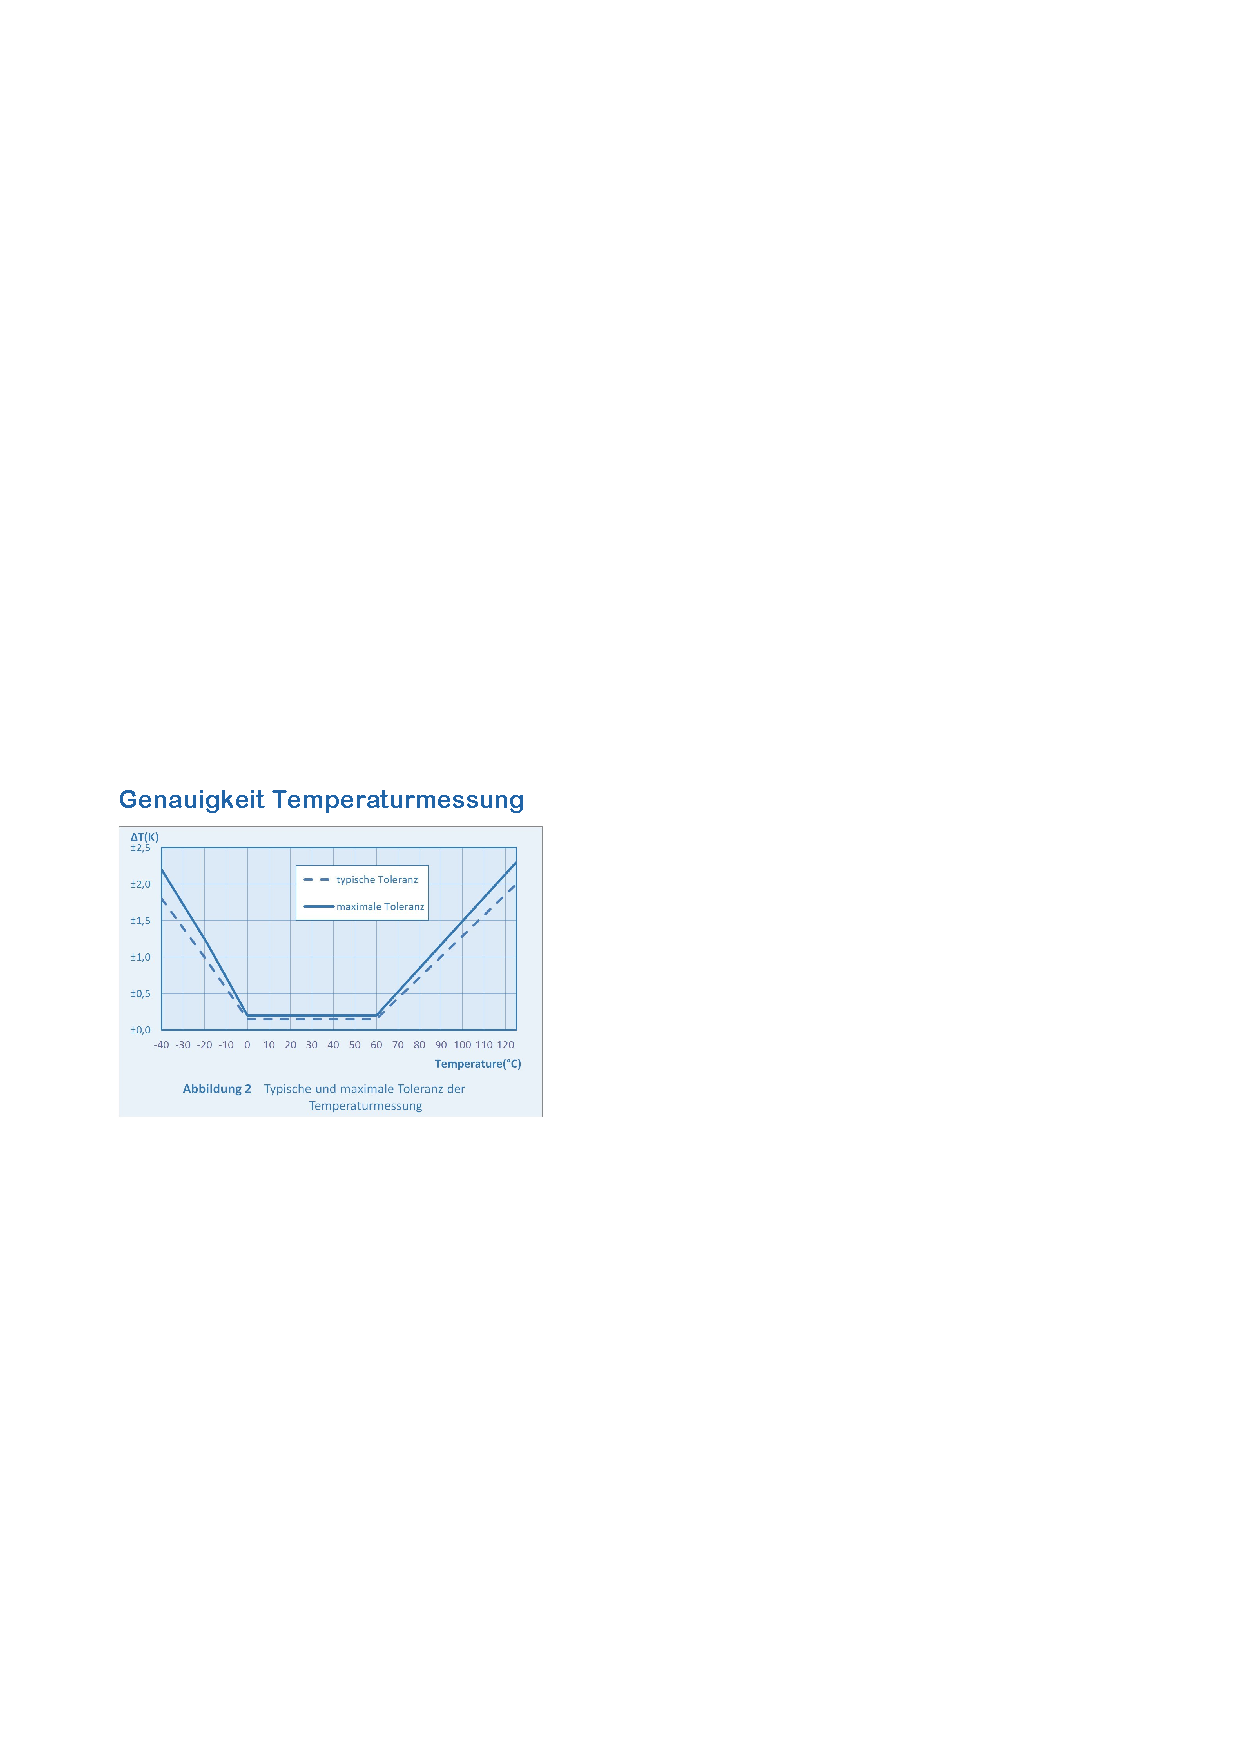
\includegraphics{./Grafiken/GenauigkeitTemp}
					\caption[Verlauf der Genauigkeit der Temperatur]{Verlauf der Genauigkeit der Temperatur\protect\footnotemark}
					\label{fig:Genauigkeit_Temp}
				\end{figure}
				\footnotetext{Quelle: \cite{HYTManual}}
				
				Der Messbereich der Feuchtigkeit beträgt 0\% bis 100\% relative Luftfeuchte. Auch hier existiert eine Ungenauigkeit, die ist mit 1,8\% angegeben ist. Die Feuchtigkeit unterliegt jedoch dem selben Effekt, dem auch die Temperatur unterliegt, der in Abbildung \ref{fig:Genauigkeit_Feuchte} dargestellt ist.
				
				\begin{figure}[H]
					\centering
					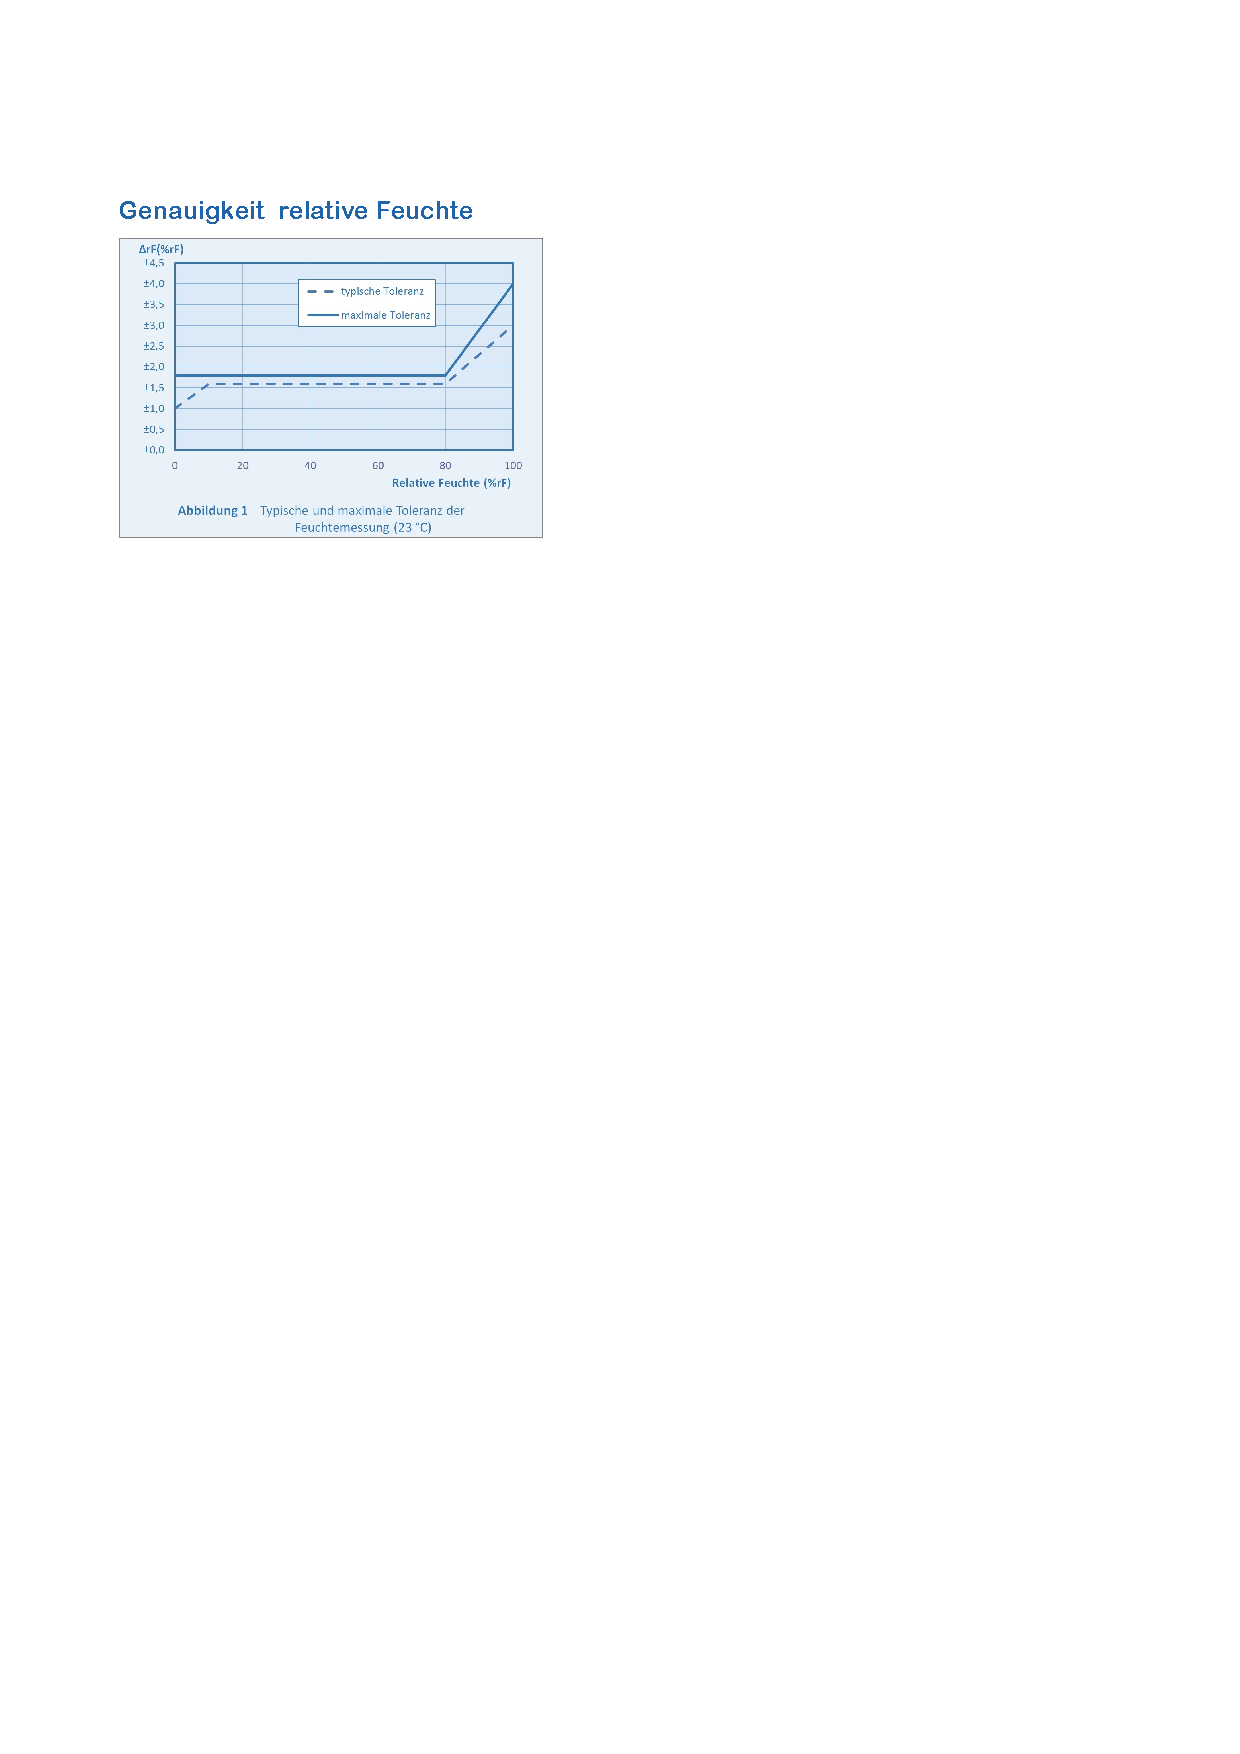
\includegraphics{./Grafiken/Genauigkeit_Feuchte}
					\caption[Verlauf der Genauigkeit der Feuchte]{Verlauf der Genauigkeit der Feuchte\protect\footnotemark}
					\label{fig:Genauigkeit_Feuchte}
				\end{figure}
				\footnotetext{Quelle: \cite{HYTManual}}
				
			\subsubsection{Technische Daten}
				\begin{table}[H]
					\centering
					\begin{tabular}{|l|l|}
					\hline Betriebsspannung & 2,7 bis 5,5 V \\
					\hline Stromaufnahme (Ruhezustand) & 1 $\mu$A \\
					\hline Stromaufnahme (Betrieb) & 850 $\mu$A \\
					\hline Schnittstellen & I²C \\
					\hline Anschlussleitungen & VCC, GND, SDA und SCL\\
					\hline
					\end{tabular}
					\caption{Technische Daten der Temperatur-/Feuchtigkeitssensoren}
					\label{table:TechHYT}
				\end{table}
			\subsubsection{Das HYT2x1 Interface}
				Die HYT271 und HYT241 Sensoren sind I$^{2}$C Slaves. Ihr Befehlssatz ist gering, aber ausreichend. Es stehen 2 Befehle zur Kommunikation zur Verfügung.
				
				\begin{description}
				\item[Measuring Request (MR)] Beim Mesuring Request wird nur auf die Adresse des Geräts geschrieben. Es müssen dabei keine Daten übertragen werden. Der reine Schreib-Befehl reicht aus.
				\item[Data Fetch (DF)] Bei Data Fetch handelt es sich um einen Lesebefehl. Hierzu muss auf den Bus die Adresse des Sensors und eine abschließende 0 gelegt werden. Folgend können vom Sensor 4 Byte empfangen und in Temperatur und Feuchtigkeit umgerechnet werden. Zwischen Data Fetch und Measuring Request sollten ca. 50ms Zeit vergehen, da sonst beim Data Fetch nur die bei vorherigen Messung ausgelesenen Werte übertragen werden.
				\end{description}
				
			\subsection{Regensensor CON-REGME-24V}
				Der vom Unternehmen B+B Thermo erworbene Sensor misst über eine mäanderförmige Leiterplatte an der Oberfläche des Moduls die Impedanz und kann daraus detektieren, ob Niederschlag vorherrscht oder nicht. Verändert sich die Leitfähigkeit zwischen den Mäandern positiv, so kann angenommen werden das es Niederschlag gibt.
				
				\newpage
				Besteht Niederschlag, so schließt oder öffnet der Sensor eigenständig ein potentialfreies Relais. Dies kann als Signalquelle frei genutzt werden. Zu beachten ist jedoch, dass keine Netzspannung mit diesem Relais geschaltet werden kann.
				
				Je nach Konfiguration des Sensors schaltet sich bei Niederschlag eine Heizung zu, die die Sensoroberfläche erwärmt. Dadurch verdunstet eventuell aufliegender Niederschlag und das Messergebnis wird deutlich genauer, da früher ein Ende des Niederschlags detektiert werden kann. Sinnvoll ist die Heizung ebenfalls im Winter, damit die Sensoroberfläche nicht vereist.
				
				Am Sensormodul selbst können noch verschiedene Einstellungen getroffen werden. Diese sind:
				
				\begin{itemize}
					\item Bei Niederschlag das Relais schließen oder öffnen
					\item Heizung verwenden oder nicht
					\item Ein optional angeschlossenes Piezoelement bei Niederschlag ertönen lassen oder abschalten
				\end{itemize}
				
				Die wichtigsten technischen Daten des Moduls sind wie folgt und können nochmals genau in dem im Lieferumfang beigelegten Datenblatt nachgelesen werden.
				
				\begin{table}[H]
					\centering
					\begin{tabular}{|l|l|}
						\hline Betriebsspannung &  24 V DC/AC +10\% \\ 
						\hline Stromaufnahme & 50 mA, Heizung 40-180 mA \\ 
						\hline Messverfahren & elektrolytische Wechselspannungsmessung \\ 
						\hline Belastung der Kontakte & max. 30 V DC / 4 A \\ 
						\hline Anschlussklemmen & 0,5 mm² - 1,5 mm² \\ 
						\hline Maße & 80 x 82 x 58 mm \\
						\hline 
					\end{tabular}
					\caption{Technische Daten des Regensensors}
					\label{table:TechRain}
				\end{table}
				
				\cite{Rain}
	\chapter{Implementierung}
	\section{Temperatur-/Feuchtigkeitssensor HYT2x1}
		\subsection{Anschluss}
			Beide Sensoren, sowohl HYT241 als auch HYT271, verfügen über vier Anschlusspins. Die zwei äußeren Pins sind VCC und GND. Die inneren Pins sind SDA und SCL, welche für die Übertragung per I$^{2}$C zuständig sind.
			
			SDA dient zur Datenübertragung. SCL ist der Taktanschluss, der standardmäßig mit einer Frequenz von 100 kHz betrieben wird. Optional hätten auch 400 kHz zur Verfügung gestanden, wurden jedoch nicht benutzt da im vorliegen Projekt keine höheren Datenraten nötig waren.
			
			Das mbed Entwicklungsboard verfügt über zwei I$^{2}$C Bus Anschlüsse. Genutzt wird der Bus auf Pin9 und Pin10. Der Schaltplan diesbezüglich kann in Abbildung \ref{fig:HYT_Schalt} betrachtet werden.
			
			\begin{figure}[H]
				\centering
				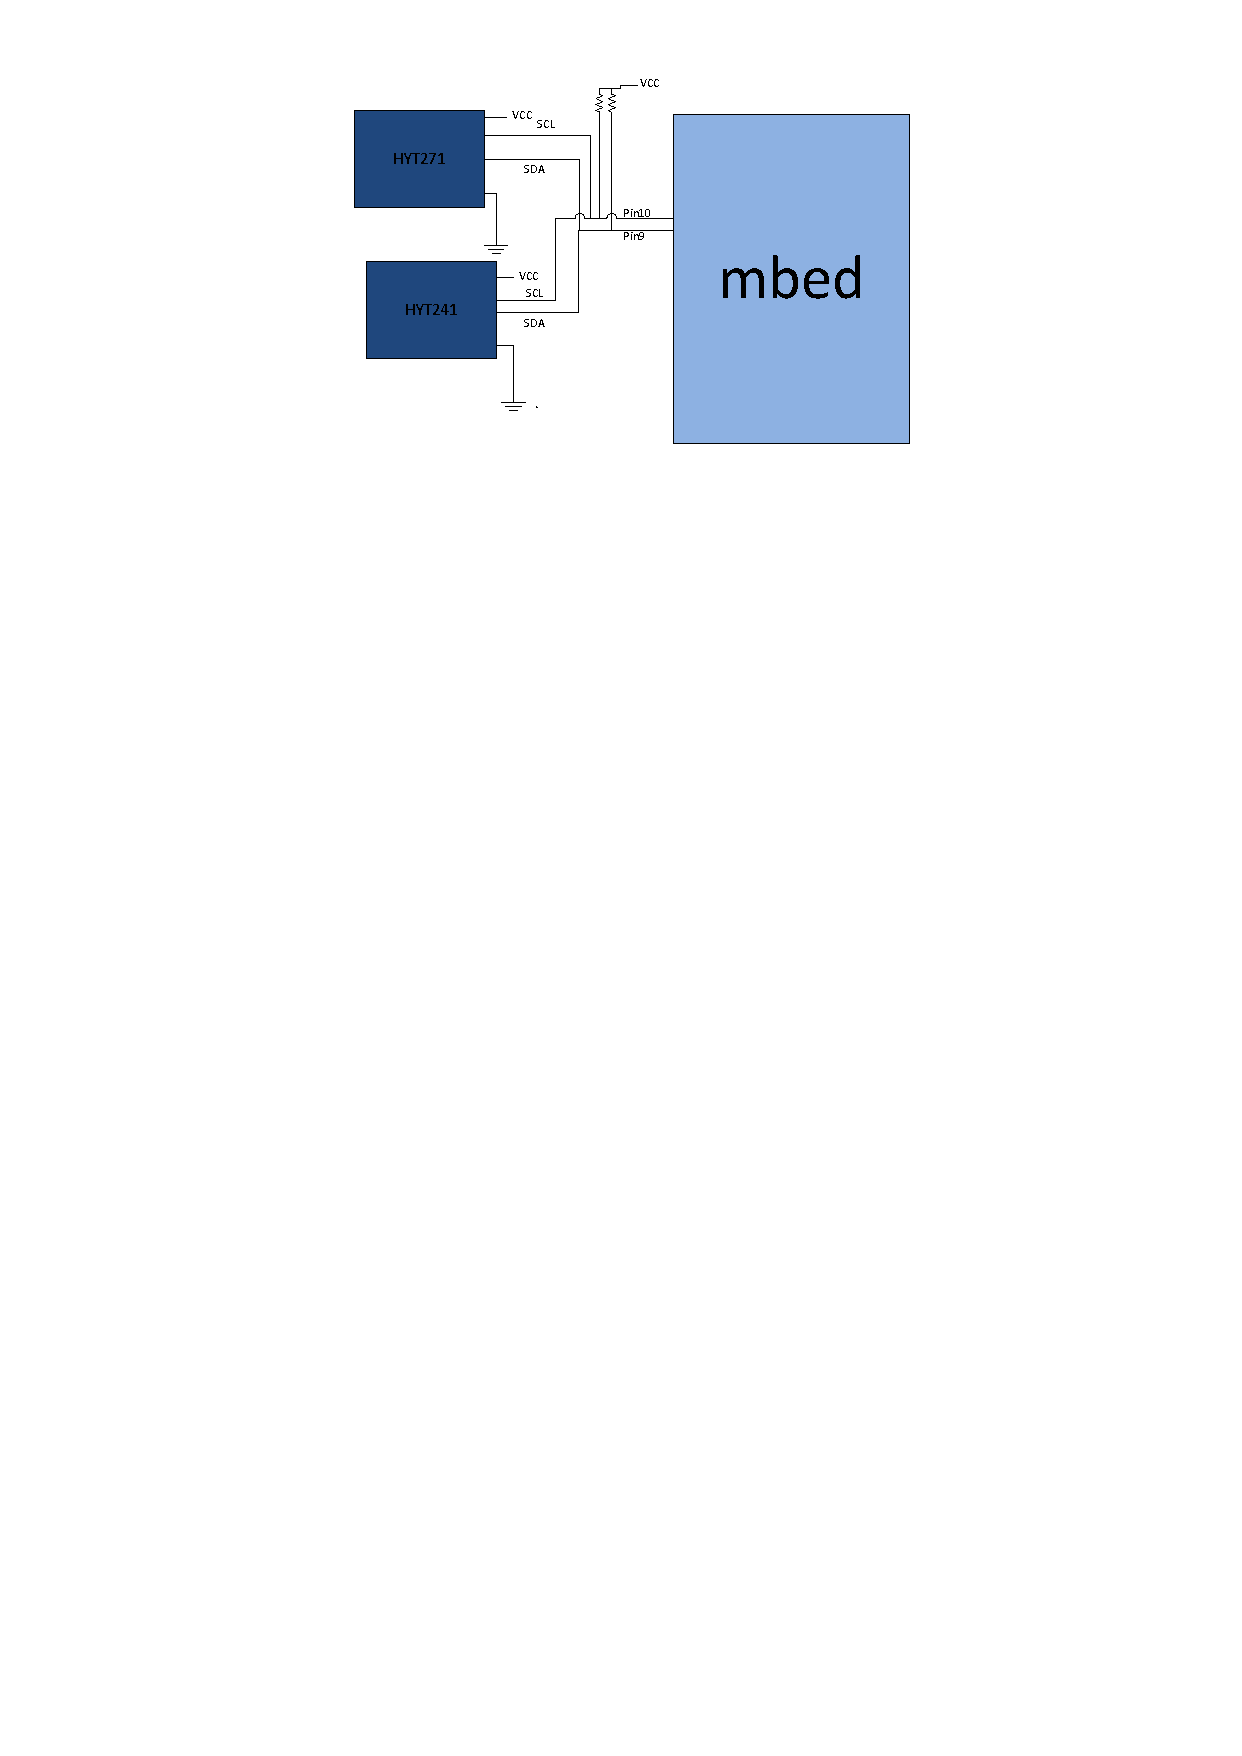
\includegraphics[width=\textwidth]{Schaltplaene/HYT_I2C}
				\caption{Schaltplan bezüglich der Temperatur-/Feuchtigkeitssensoren}
				\label{fig:HYT_Schalt}
			\end{figure}

		\subsection{Adressen}
			Im Projekt werden zwei Sensoren über einen Bus angesteuert. Das heißt, dass beide Sensoren mit Pin9 und Pin10 verbunden sind. Sie besitzen allerdings die gleiche Standardadresse 0x28. Damit beide Sensoren korrekt arbeiten musste die Adresse des HYT241 auf 0x20 geändert werden. Die extra Schaltung, die hierfür nötig war ist in Abbildung \ref{fig:HYT_Schalt_Umprog} zu sehen.
			
			\begin{figure}[H]
				\centering
				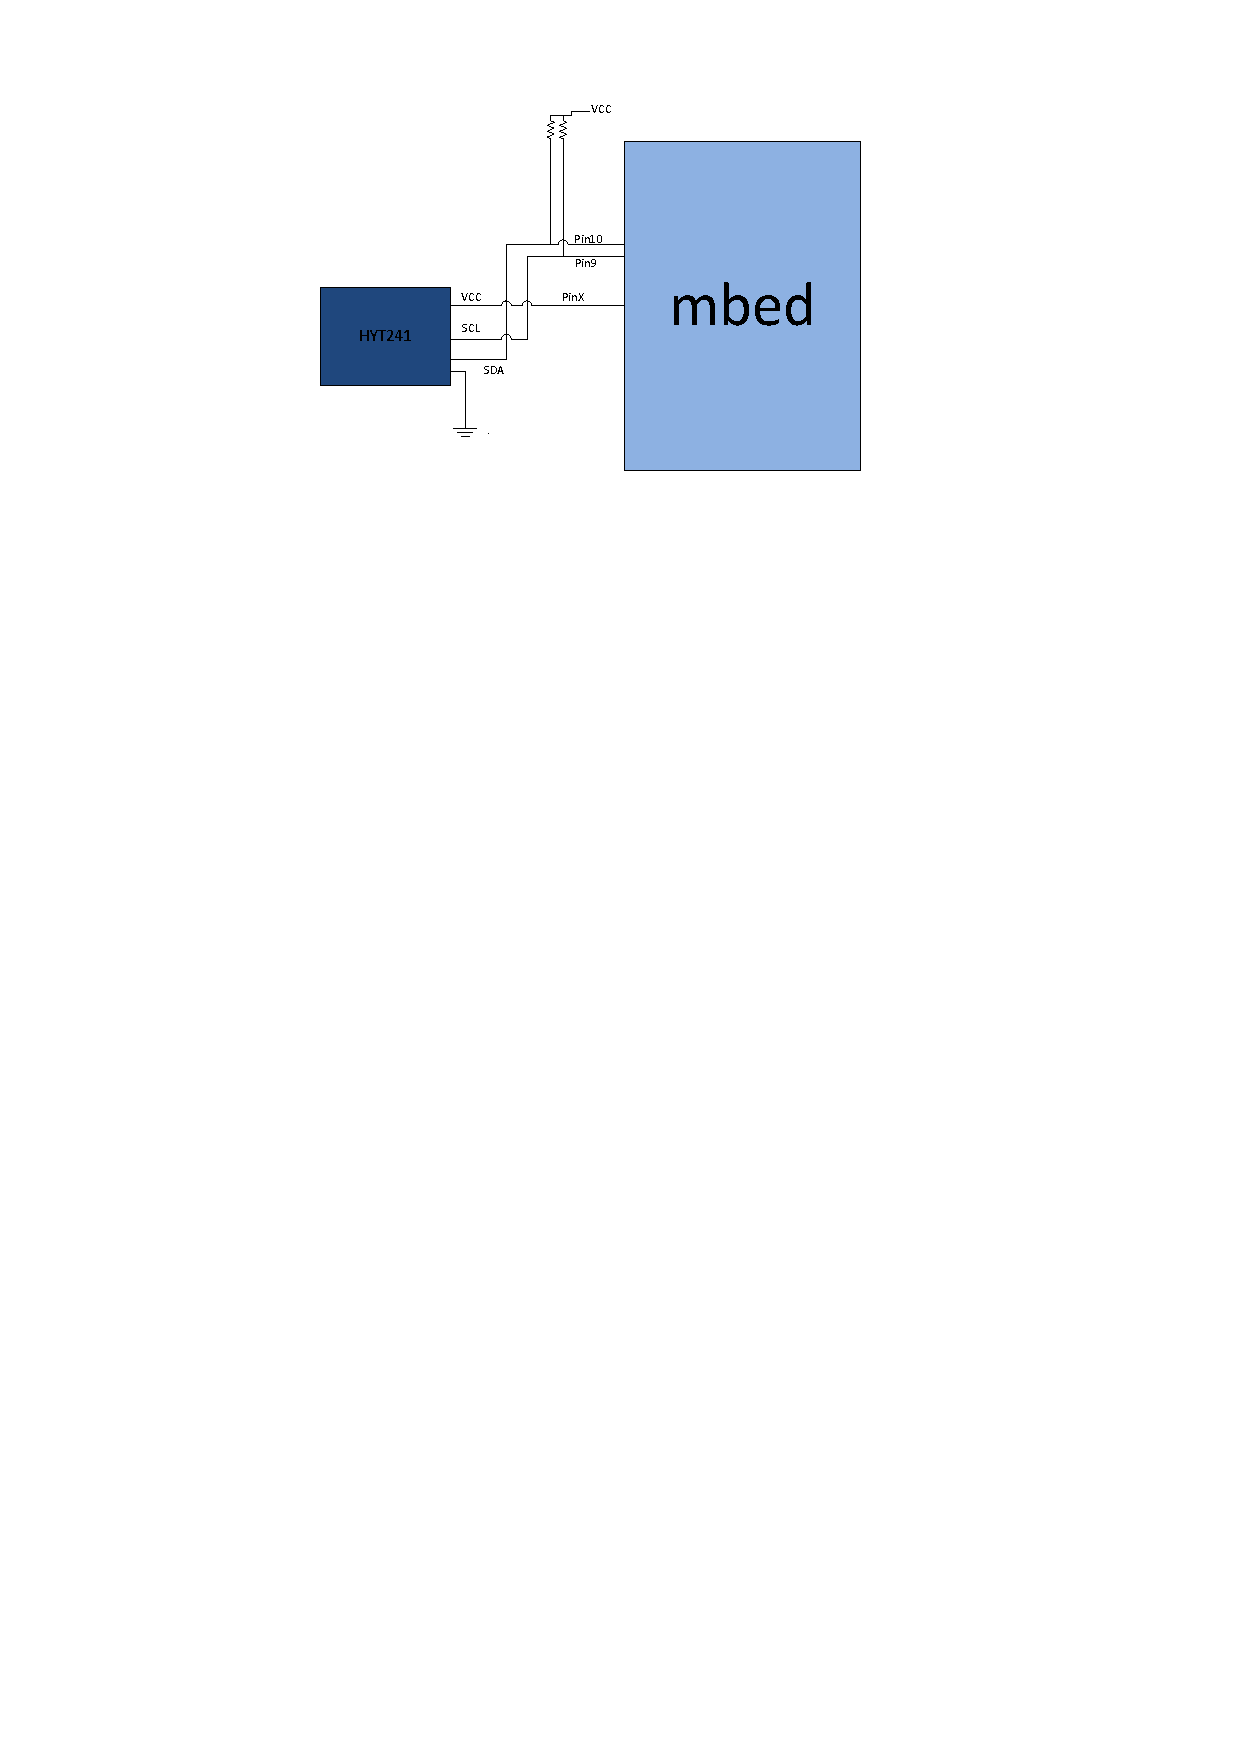
\includegraphics[width=\textwidth]{Schaltplaene/Umprogrammieren}
				\caption{Schaltplan bezüglich der Adressänderung}
				\label{fig:HYT_Schalt_Umprog}
			\end{figure}

			\subsubsection{Das Adressänderungsprotokoll}
			Innerhalb der ersten 10 ms nach dem einschalten des Sensors kann dieser in den Programmiermodus gesetzt werden. Da dieses Zeitfenster mit dem mbed Entwicklungsboard jedoch schlecht zu treffen ist musste zum verändern der Adresse die Schaltung selbst verändert werden, damit der Sensor separat eingeschaltet werden kann.
			
			Zunächst muss der VCC Pin des Sensors mit einem beliebigen freien Pin des mbed Prototypboards verbunden werden. Dann kann die Methode setAdress() der HYT2x1 Klasse aufgerufen werden.
			
			\newpage
			Durch das Aufrufen der setAdress() Methode wird der VCC Pin des Sensors auf High\footnote{Eigentlich reichen Logikausgänge nicht aus um Sensoren mit Strom zu versorgen, da ihre Leistung schlicht zu gering ist. Im Falle des HYT241 spielt das jedoch keine Rolle. Dieser ist so sparsam ausgelegt das auch ein Logikausgang ausreicht um ihn mit Strom zu versorgen.} gelegt. Durch das Anlegen des High-Signals wird der Sensor eingeschaltet und man kann ihn in den Programmiermodus setzen. Dazu muss der Befehl \{0xA0,0x00,0x00\} auf die bisherige Adresse des Sensors geschrieben werden. Da man dem Sensor etwas Zeit geben muss den Befehl zu bearbeiten, wird anschließend 100ms gewartet. Dann kann der nächste Befehl gesendet werden. Dieser lautet \{0x5C,0x00,Adresse\footnote{Die neue Adresse im Hexadezimalen Format.}\}. Folgend muss erneut 100ms gewartet werden. Jetzt muss nur noch der letzte Befehl zum Bestätigen der Adresse gesendet werden, der \{0x80,0x00,0x00\} lautet. Nun wurde die Adresse des Sensors geändert, wodurch er nicht mehr auf die alte Adresse reagiert.
			
			Anmerkung: Dieses Protokoll steht nicht im Datenblatt des Sensors und wurde über mehrere Forenbeiträge aus dem Internet zusammengetragen. Den Aussagen zufolge wurde dieser Algorithmus per Reverse-Engeneering herausgefunden.
		\subsection{Messen mittels HYT271/HYT241}
			In der HYT2x1 Klasse ist die update() Methode implementiert. Diese Methode kapselt den Messbefehl und kommt ohne Parameter aus. Alle nötigen Informationen zum Messen befinden sich in den zuvor erzeugten HYT2x1 Objekten.
			
			Die update() Methode startet einen Schreibbefehl auf die Adresse des Sensors. Die Adresse muss um 1 Bit nach links geschoben werden. Nun wird automatisch eine 1 an die Adresse angehängt. Dies geschieht über das I$^{2}$C Interface der mbed Standardbibliothek.
			
			Nun wird 50ms gewartet damit der Sensor seine Messung durchführen kann. Danach wird ein Lesebefehl auf die Adresse des Sensors ausgeführt. Jetzt werden vier Byte gelesen und in dem Objekt gespeichert. Die ersten beiden Bytes geben die relative Luftfeuchtigkeit und die letzten beiden die Temperatur an.
			\subsubsection{Die Temperatur auslesen}
				Nach der update() Methode kann die getTemp() Methode aufgerufen werden. Diese Methode gibt die aktuell gemessene Temperatur als Gleitkommazahl zurück. Im eigentlichen  Objekt liegt sie allerdings als Byte Wert vor. Um den Byte Wert in eine Gleitkommazahl zu konvertieren muss folgende Formel benutzt werden:
				
				\[ h = (Highteil << 6) | Lowteil >> 2) \]
				\[ t = ((165.0 / 16384) * h) - 40.0 \]
				
			\cite{HYTManual}
			\subsubsection{Die relative Luftfeuchtigkeit auslesen}
				Nach der update() Methode kann auch die getHumid() Methode aufgerufen werden. Diese Methode gibt die im letzten Messvorgang gemessene relative Luftfeuchtigkeit als Gleitkommazahl zurück. In dem Objekt liegt sie aber noch als Byte Wert vor. Um den Byte Wert in eine Gleitkommazahl zu konvertieren muss Folgende Formel benutzt werden:
				
				\[ h1 = ((Highteil \& 0x3F) << 8) | Lowteil \]
				\[ h = (100.0 / 16384) * h1 \]
				
				\cite{HYTManual}
	\section{Empfangsmodul DCF77}
		\subsection{Übertragungsprotokoll}
			Das aus Mainhausen ausgesendete Langwellensignal wird mit einer Frequenz von 77,5 kHz betrieben. Innerhalb einer Minute werden über dieses Signal 59 Informationsbits übertragen, aus denen unter anderem die Uhrzeit dekodiert werden kann.
			
			Die Übertragung der Informationen erfolgt über eine negative Modulation des Signals im Sekundentakt. Die Trägeramplitude wird innerhalb einer Sekunde im Bereich von 100 bis 200 ms auf 15\% ihrer Ausgangsleistung abgesenkt. Über eine entsprechende Schaltung (in Abbildung \ref{fig:DCF77-Plan} dargestellt) an der Empfangsantenne kann dies auf logische Pegel Übertragen werden, die man am Eingang eines Chips auslesen kann. Damit liegt pro Sekunde zwischen 100 und 200 ms eine logische Null am Eingang an.
			
			\begin{figure}[H]
				\centering
				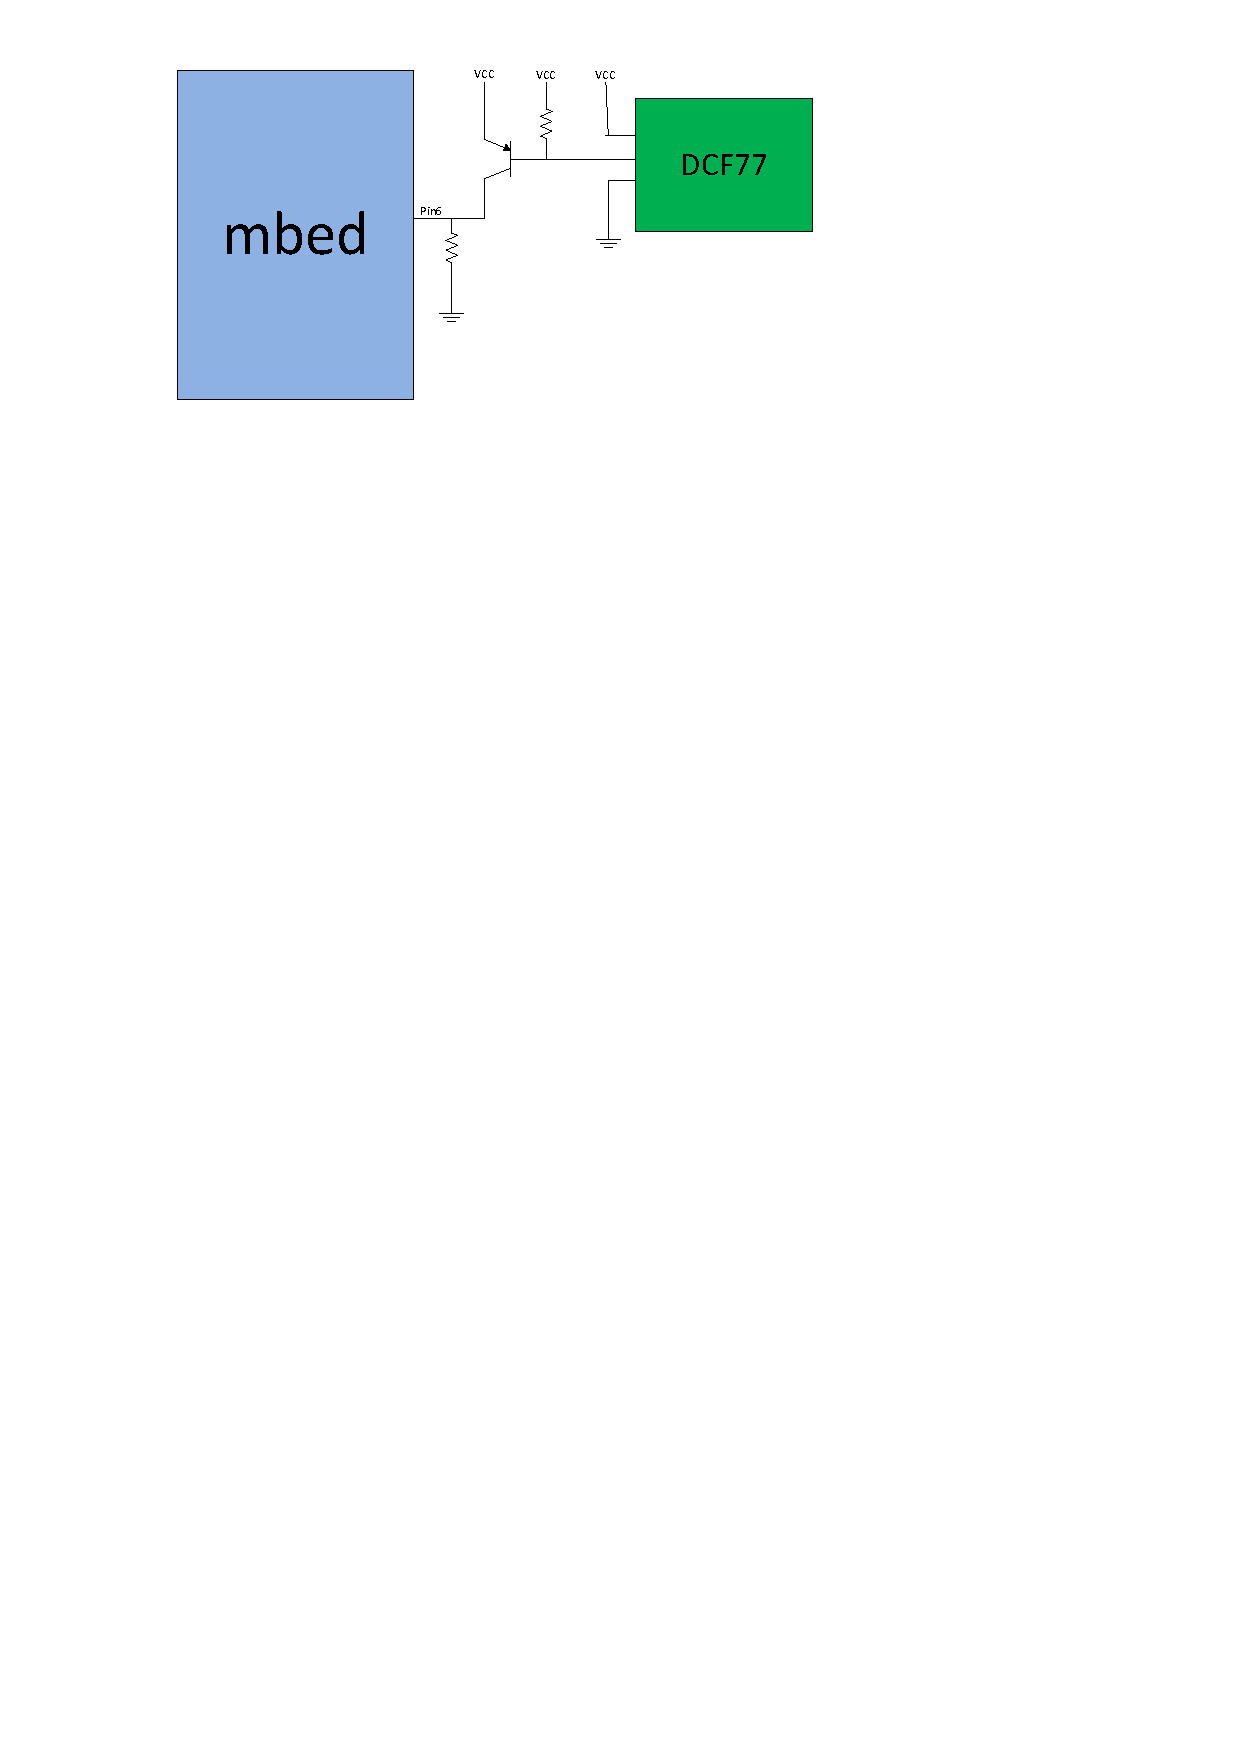
\includegraphics[width=\textwidth]{Schaltplaene/DCF77_Schaltung}
				\caption{Schaltplan DCF77}
				\label{fig:DCF77-Plan}
			\end{figure}

%			\begin{figure}[H]
%				\centering
%				\includegraphics[width=0.7\linewidth]{Schaltplaene/DCF77}
%				\caption{Schaltplan DCF77}
%				\label{fig:DCF77-Plan}
%			\end{figure}
			
			\newpage
			Zum Ende jeder Minute fehlt eine dieser logischen Nullen. Diese lange logische eins (2 s) markiert den Beginn einer neuen Übertragung. Folgend wird zum Beginn jeder Sekunde ein Informationsbit übertragen. Eine Entscheidung, ob das Bit einer eins oder einer null entspricht, geschieht über die Länge der anliegenden logischen null. Liegt diese bei 100 ms, so ist dies als 0 zu interpretieren. Liegt diese bei 200 ms, so ist dies als 1 zu interpretieren. Damit ist das Protokoll ähnlich zum 1-Wire Protokoll, jedoch deutlich einfacher.
			
			Ein entsprechender Verlauf des Signals ist in Abbildung \ref{fig:DCF77_Impulse} zu sehen.
			
			\begin{figure}[H]
				\centering
				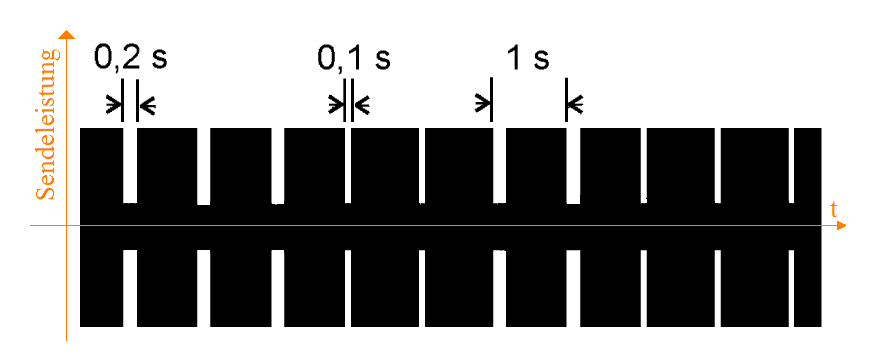
\includegraphics[width=12cm]{Grafiken/DCF77_Impulse}
				\caption[Amplitudenmodulierte Sendeleistung als Funktion der Zeit]{Amplitudenmodulierte Sendeleistung als Funktion der Zeit\protect\footnotemark}
				\label{fig:DCF77_Impulse}
			\end{figure}
			\footnotetext{Quelle: \cite{DCF77Wiki}}
			
			Letztlich können so über eine Minute 59 Bits an Informationen empfangen werden, ehe mit der langen logischen 1 ein erneuter Übertragungszyklus beginnt.
			
			\cite{DCF77Wiki}
		\subsection{Übertragene Informationen}
			In denen vom Sender ausgestrahlten 59 Bits sind kodiert verschiedene Informationen enthalten:
			
			\newpage
			\begin{itemize}
				\item Wetterinformationen der Firma MeteoTime
				\item Informationen zum Katastrophenschutz
				\item MEZ oder MESZ
				\item Uhrzeit
				\item Datum
				\item Am Ende der Stunde wird MEZ/MESZ umgestellt
				\item Am Ende der Stunde wird eine Schaltsekunde eingefügt
			\end{itemize}
			
			Die Wetterinformationen sowie die Informationen zum Katastrophenschutz sind dabei verschlüsselt und müssen über einen erwerbbaren Schlüssel dekodiert werden. Die restlichen Informationen (Uhrzeit, Datum) sind als BCD-Zahlen kodiert.
			
			Bezüglich der Uhrzeit werden die Minuten und Stunden des aktuellen Tages übertragen. Die aktuellen Sekunden können über den Beginn der Übertragung herausgefunden werden, da diese immer zur Sekunde null beginnt.
			
			Bezüglich des Datums werden der Kalendertag, der Wochentag, die Monatsnummer und das Jahr übertragen.
			
			\cite{DCF77Wiki}
		\subsection{Auswertung der Informationen}
			Die Bits samt ihren Bedeutungen sind der im Anhang dargestellten Tabelle \ref{table:DCF77Frame} zu entnehmen.
			
			Bits 0 bis 15 können dabei ignoriert werden, sofern man den für diese Informationen benötigten Schlüssel nicht besitzt.
			Die Bits 16 bis 19 können direkt ausgewertet werden, ohne eine Dekodierung vornehmen zu müssen.
			
			Letztlich muss noch das Datum und die Uhrzeit ausgewertet werden. Diese Informationen sind BCD kodiert. Am Beispiel der Minute wird gezeigt, wie diese zu dekodieren sind.
			
			Wird die Bitreihenfolge \enquote{1100101} als Bits 21 bis 27 empfangen so können hieraus die in der aktuellen Stunde verstrichenen Minuten dekodiert werden. Entsprechend der Kodierung wird jedem Bit eine spezielle Dezimalzahl zugeordnet. Die Bits müssen nun nur entsprechend der Zuordnung multipliziert werden, um die Uhrzeit herauszufinden. Am Beispiel der obigen Reihenfolge:
			
			\[ 1*1+1*2+0*4+0*8+1*10+0*20*1*40 = 53 \]
			
			Somit steht die Reihenfolge \enquote{1100101} der Bits 21 bis 27 für die Minute 53.
			
			Für die Minuten, Stunden sowie das gesamte Datum existieren jeweils Prüfbits. Diese stellen Paritätsbits einer positive Paritätsprüfung dar. Zusätzlich zu dieser schwachen Überprüfung auf Übertragungsfehler kann nach dem Dekodieren der einzelnen Datenfelder noch geprüft werden, ob diese im richtigen Wertebereich vorliegen. Am Beispiel der Minuten muss überprüft werden, ob diese im Bereich 0 bis 59 liegen.
			
			Hat die Prüfung alle Instanzen erfolgreich durchlaufen kann man relativ sicher sein, die richtigen Informationen erhalten zu haben. Sollte man den Fehler weiter minimieren wollen, so muss man mehrere Minuten das Signal empfangen und dann entsprechend vergleichen, ob jeder empfange Bitstrom gleiche Datenstempel (mit entsprechend veränderter Minute) liefert.
			
			\cite{DCF77Wiki}
		\subsection{Besonderheiten der Implementierung}
			Dadurch, dass das Signal wenigstens 38 Sekunden empfangen werden muss um eine gültige Uhrzeit zu bestimmen, wurde das gesamte Programm auf eine minimale Systemlast optimiert. Dies umfasst den besonders kritischen Empfang des Bitstrom, aber auch die Minimierung der Speicherlast.
			
			Der Empfang des Bitstroms erfolgt über Interrupts an einem Eingangspin. Diese sind so arrangiert, dass bei fallender Flanke ein Timer gestartet wird, der bei steigender Flanke angehalten und ausgewertet wird. Hat dieser Timer eine Zeit zwischen 50 und 250 ms aufgenommen, so wird das Bit entsprechend der Vorschrift geschaltet. Lief der Timer kürzer oder länger, so wird ein Fehlerfall geschaltet. Dieser kann beispielsweise auftreten, wenn schlechter Empfang vorherrscht.
			
			Diese Implementierungsart ist grundsätzlich einer Benutzung von \enquote{wait()} vorzuziehen, da mit der wait-Funktion der komplette Prozessor blockiert wird. Die Funktion \enquote{Thread::wait()} bzw. die Benutzung von Semaphoren ist hier eindeutig vorzuziehen, da diese nur den aktuellen Thread blockieren.
			
			Solange der Bitstrom (59 Bits) empfangen wird, wird die Ausführung des eigentlich aufrufenden Programms über einen Semaphor blockiert. Es sollte also darauf geachtet werden diesen Sensor in einem extra Thread laufen zu lassen, welcher blockieren kann ohne die restliche Programmausführung zu behindern.
			
			Entsprechend der Dokumentation wird am Bitstrom eine Paritätsprüfung vorgenommen. Ist diese erfolgreich, werden die Daten dekodiert und nochmals bezüglich des Wertebereichs geprüft. Lief auch hier alles erfolgreich durch, kehrt der Funktionsaufruf mit einem \enquote{true} zurück. Trat wider erwarten ein Fehler auf, wird der Empfang maximal drei mal wiederholt, ehe der Funktionsaufruf mit einem \enquote{false} zurückkehrt.
			
			Die erfolgreich gewandelte Uhrzeit kann nun über eine Funktion abgerufen werden. Mit dieser erhaltenen Information kann über eine weitere Funktion die interne \enquote{Real-Time-Clock} gesetzt werden.
	\section{Regensensor CON-REGME-24V}
		\subsection{Auswertung der Informationen}
			Der Sensor liefert nur eine sehr einfache Information. Es wird lediglich über das potentialfreie Relais bereitgestellt, ob Niederschlag vorherrscht oder nicht.
		\subsection{Besonderheiten der Implementierung}
			Der Sensor wird, sobald initialisiert, genau wie der DCF77 Schaltkreis über einen Interrupt-Pin abgefragt. Bei einer steigenden Flanke setzt das Programm intern den Wert dafür, das es Regnet auf \enquote{true}, bei einer fallenden Flanke auf \enquote{false}.
			
			Diese Vorgehensweise verringert genau wie beim Programm für den DCF77 Schaltkreis die Systemlast zu einer aktiven Abfrage enorm und der interne Zustand ist unabhängig von den Aufrufbedingungen immer aktuell.
			
			Über eine entsprechend bereitgestellte Funktion kann der aktuelle Zustand abgefragt werden.
	\section{Logging}
		\subsection{Die Logging Klasse}
		Um die empfangenen Sensordaten zu speichern und später auszuwerten wurde eine Logging-Funktion implementiert. Hierzu wurde keine neue Hardware verbaut, es handelt sich um eine reine Softwarelösung. Auf dem mbed-Entwicklungsboard befindet sich ein 2 MByte großer Flash-Speicher, der zum Protokollieren der Messwerte ausreicht.
		
		Um auch die Logging-Funktion zu kapseln wurde eine Logging-Klasse erstellt. Nach dem Erstellen eines Logging-Objektes muss nur die log() Methode aufgerufen werden um etwas zu speichern. Mit dem Erstellen eines Log-Objektes wird automatisch ein Filepointer auf die Datei \enquote{LOG.txt} geöffnet. Beim Zerstören des Objektes wird dieser wieder geschlossen.
		\subsection{Puffer Funktion}
		Ein Flash-Speicher hat nur eine begrenzte Anzahl an Schreibvorgängen pro Speicherzelle. Um diese Schreibzyklen optimal auszunutzen, wurde darauf geachtet die Schreibzugriffe gering zu halten und zugleich möglichst viel auf einmal zu schreiben.
		
		Der Flash-Speicher wurde auf 512 Byte-Blöcke formatiert. Diese werden, wenn möglich, mit einem mal voll beschrieben. Die zu schreibenden Daten werden im RAM des mbed Entwicklungsboards zwischengespeichert. Wenn über 450 Byte Gesamtgröße des Pufferarrays erreicht sind wird der gesamte Pufferspeicher auf den Flash-Speicher geschrieben.
	\chapter{Protokolle}
	\section{Regensensor CON-REGME-24V}
		Im Datenblatt wurde bezüglich des Regensensors CON-REGME-24V eine maximalen Stromaufnahme von 230 mA angegeben. Als der Regensensor in Betrieb genommen wurde fiel auf, dass er mehr als angeben benötigt. Aus diesem Grund wurde eine Messreihe diesbezüglich aufgenommen und einen Grund für das Verhalten zu ermitteln.
		
		\begin{table}[H]
			\centering
			\begin{tabular}{|l|l|l|}
				\hline \textbf{Max Ampere} & \textbf{Erster Testlauf} & \textbf{Zweiter Testlauf}\\
				\hline 1,5A& 10ms & 5ms\\
				\hline 1,0A& 10ms & 10ms\\ 
				\hline 0,75A& 15ms & 14ms\\ 
				\hline 0,5A& 25ms & 27ms\\ 
				\hline 0,3A& 57ms & 53ms\\ 
				\hline 0,3A& nicht ermittelbar & nicht ermittelbar\\
				\hline
			\end{tabular}
			\caption{Abbauzeiten bzgl. der Strombegrenzung des Regensensors}
			\label{table:RainmA}
		\end{table}
		
		In der Tabelle \ref{table:RainmA} wird dargestellt, wie lang die Stromversorgung in die Strombegrenzung geht, sobald der Strom eingeschaltet wird. Der Effekt tritt allerdings nur auf, wenn man den Sensor in Verbindung mit der eingebauten Heizung verwendet.
		
		Es kann nur vermutet werden, das die ermittelten Werte auf den Kaltleitereffekt der Heizung zurückzuführen sind. Dieser Effekt gibt an, das der Widerstand des Leiters im kalten Zustand relativ gering ist und sich bei Erwärmung deutlich erhöht. Somit würde über den Leiter, bis er sich erwärmt hat, ein hoher Strom fließen.
		
		In den folgenden Abbildungen sieht man die genauen Oszilloskop-Messergebnisse.
		
		\begin{figure}[H]
		\centering
		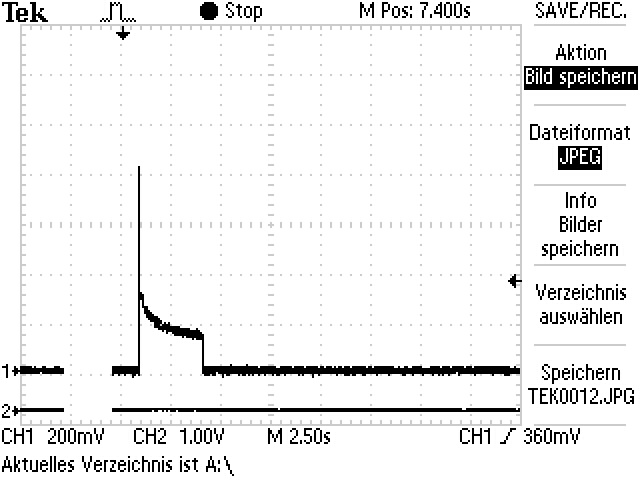
\includegraphics[width=10cm,height=5cm]{./Grafiken/TEK0012}
		\caption{Messung bei einer Strombegrenzung von 1,5A}
		\label{fig:TEK0012}
		\end{figure}
		
		\begin{figure}[H]
		\centering
		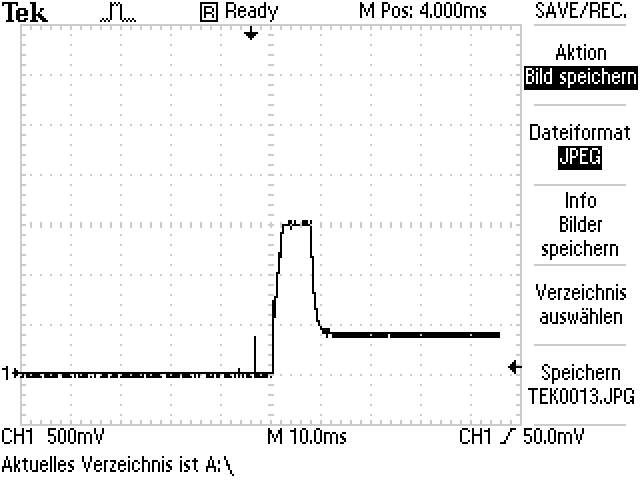
\includegraphics[width=10cm,height=5cm]{./Grafiken/TEK0013}
		\caption{Messung bei einer Strombegrenzung von 0,5A}
		\label{fig:TEK0013}
		\end{figure}
		
		\begin{figure}[H]
		\centering
		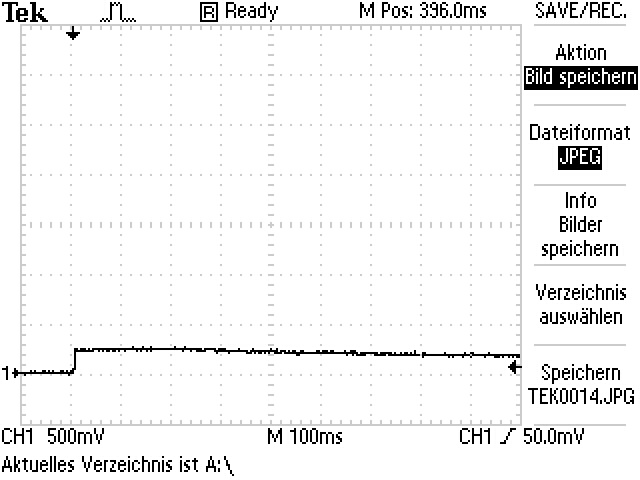
\includegraphics[width=10cm,height=5cm]{./Grafiken/TEK0014}
		\caption{Messung bei einer Strombegrenzung von 0,23A}
		\label{fig:TEK0014}
		\end{figure}
		
		In der letzten Abbildung \ref{fig:TEK0014} war der Unterschied zwischen Strombegrenzung und Leistungsaufnahme so gering, dass kein Zeitpunkt bestimmt werden konnte, ab dem die Heizung auf Betriebstemperatur ist. Deswegen kann in der Tabelle \ref{table:RainmA} kein Wert angegeben werden.
		
		Als Resultat muss der Sensor, sofern er mit der integrierten Heizung verwendet wird, über eine separate Spannungsversorgung betrieben werden. Wäre dies nicht der Fall, so würde ein Spannungszusammenbruch die gesamte restliche gekoppelte Elektronik beeinflussen. Alternativ muss extra für diesen Sensor eine Strombegrenzung eingesetzt werden, die die Spannung in der Restschaltung konstant hält.
	\section{Feuchte-/Temperatur Sensoren HYT271/241}
		Um bezüglich dieser Sensoren eine Aussage über die Genauigkeit geben zu können, wurde eine Reihe von Messungen durchgeführt. Um einen Referenzwert bezüglich der gelieferten Sensordaten geben zu können wurden zwei weitere Geräte verwendet. Einerseits das Klimalogg Pro\footnote{Etwa 100\euro{}} und andererseits das Medbus\footnote{Etwa 10\euro{}}.
		
		Da die Messungen allerdings nur exemplarisch durchgeführt wurden und dies nicht in einer Klimakammer mit speziellen Messbedingungen erfolgte, kann mit den folgenden Ergebnissen keine exakte Aussage getroffen werden. Es kann lediglich grob abgeschätzt werden, ob die Sensoren bezüglich der Referenzgeräte exakt arbeiten.
		\subsubsection{Messergebnisse bezüglich der relativen Luftfeuchtigkeit}
		
		\begin{table}[H]
			\centering
			\begin{tabular}{|l|l|l|l|l|}
				\hline \textbf{Ort der Messung} & \textbf{HYT271} & \textbf{HYT241} & \textbf{Medbus} & \textbf{Klimalogg Pro}\\
				\hline Arbeitszimmer & 45,2 & 46,1 & 51 & 52 \\
				\hline Balkon & 53,5 & 55,0 & 49 & 60 \\
				\hline Kühlschrank & 59,3 & 62,8 & 50 & 53 \\
				\hline Schrank & 57,2 & 58,1 & 49 & 49 \\
				\hline Badezimmer & 68,5 & 71,7 & 55 & 65 \\
				\hline 
			\end{tabular}
			\caption{Messergebnisse bezüglich der relativen Luftfeuchtigkeit (in \%)}
			\label{table:HYTHumid}
		\end{table}
		
		Man kann anhand den Daten sehen, das die Messwerte der Sensoren in der selben Größenordnung der Referenzgeräte liegen. Es sind allerdings auch deutliche Abweichung zu erkennen. Ohne Tests in einer Klimakammer kann hierzu allerdings keine weitere Aussage getroffen werden.
		
		\subsubsection{Messergebnisse bezüglich der Temperatur}
		
		\begin{table}[H]
			\centering
			\begin{tabular}{|l|l|l|l|l|}
				\hline \textbf{Ort der Messung} & \textbf{HYT271} & \textbf{HYT241} & \textbf{Medbus} & \textbf{Klimalogg Pro}\\
				\hline Arbeitszimmer & 20,6 & 20,8 & 19,5 & 19,7 \\
				\hline Balkon & 5,7 & 6,1 & 7,2 & 5,7 \\
				\hline Kühlschrank & 8,4 & 8,5 & 9,1 & 9,5 \\
				\hline Schrank & 17,0 & 17,6 & 19,1 & 19,1 \\
				\hline Badezimmer & 19,7 & 20,3 & 19,8 & 20,6 \\
				\hline
			\end{tabular}
			\caption{Messergebnisse bezüglich der Temperatur(in °C)}
			\label{table:HYTTemp}
		\end{table}
		
		Bezüglich der Temperatur passen die Messergebnisse deutlich besser als bei der relativen Luftfeuchte. Jedoch ist auch hier eine sehr große Abweichung zu erkennen. Es gilt ebenfalls, das ohne Tests in einer Klimakammer keine weiteren Aussagen getroffen werden können.
	\chapter{Zusammenfassung}
	\section{Ergebnis der Arbeit}
		Das Ziel der Arbeit bestand darin, verschiedene Sensoren zur Umwelterfassung zu bewerten und eine Referenzimplementierung auf der Plattform mbed NXP LPC1768 bereitzustellen.
		
		Es wurden zwei Sensoren zur Temperatur-/Luftfeuchteerfassung bereitgestellt, ein Empfänger um das allgemein ausgestrahlte Zeitsignal DCF77 zu empfangen und ein Sensor, der Regen detektieren kann. Für all diese Sensoren wurde eine Referenzimplementierung in C++ geschaffen, damit diese möglichst einfach in Projekten benutzt werden können. 
		
		Bei dieser Implementierung wurde auf eine möglichst geringe CPU-Last wert gelegt, da die Erfassung von Umweltdaten nicht das einzige Ziel des Mikrocontrollers darstellt. Ohne eine detaillierte Debugging-Möglichkeit kann jedoch nicht festgestellt werden, wie gut dies gelungen ist und kann nur theoretisch abgeschätzt werden.
		
		Die verwendeten Temperatur-/Luftfeuchtesensoren funktionieren anhand der Testergebnisse sehr gut, besitzen jedoch, im Vergleich zu einem teurem Messgerät, deutliche Abweichungen. Die Referenzimplementierung bietet die Möglichkeiten den Sensor abzufragen und folgend einzeln die Temperatur und Luftfeuchte zu erfragen. Auch ein ändern der Adresse des Sensors bezüglich des I²C Protokolls ist möglich, erfordert jedoch eine spezielle Vorschaltung.
		
		\newpage
		Der Regensensor detektiert zuverlässig, ob Niederschlag vorherrscht oder nicht. Mit der verfügbaren Empfindlichkeitseinstellung kann dieser so weit verändert werden, das selbst Nebel erkannt werden kann. Der Sensor hat jedoch scheinbar ein Problem innerhalb der Verschaltung, da er einen deutlich höheren Maximalstrom als im Datenblatt angegeben benötigt. 
		
		Das Empfangsmodul für das DCF77 Signal empfängt das ausgestrahlte Signal zuverlässig, sofern das Modul speziell ausgerichtet ist und sich nicht in der Nähe von Störquellen befindet. Sind diese beiden Punkte doch eingetreten, so wird der korrekte Empfang des Signals fast unmöglich. Die Implementierung für den Empfänger bietet separat an den aktuellen Uhrzeitstempel zu empfangen, diesen auszulesen und die Controller interne \enquote{Real-Time-Clock} zu setzen. Um Empfangsschwierigkeiten erfassen zu können wurde eine intensive Überprüfung des empfangen Stempels implementiert.
	\section{Bewertung des Ergebnisses}
		\subsection{DCF77 Empfänger}
			Der Empfänger für das Signal DCF77 liefert zuverlässig das aus Mainhausen ausgestrahlte Funksignal und hat sich mit kleineren Problemen gut benutzen lassen. 
			
			Eines der Probleme stellt die eher dürftige Dokumentation des Empfängers dar. Die über Conrad bereitgestellten Dokumente beschreiben den Empfänger nur sehr schlecht und die Informationen diesbezüglich musste über Foren und Erfahrungsberichte zusammengetragen werden. Da diese jedoch keine zuverlässige Quelle darstellen und man nicht genau sagen kann, was die entsprechenden Autoren eventuell anders als im vorliegenden Projekt gemacht haben, sind diese Informationen eher als kritisch zu bewerten.
			
			Eines der Dokumentationsprobleme lag im Anschluss des Empfängers an den Mikrocontroller. Es ist zwar ein Schaltplan auf der Internetseite von Conrad gegeben, es war jedoch nicht ersichtlich warum diese Schaltung benutzt werden muss. Da ohne die entsprechende Schaltung aber kein stabiles Signal am Mikrocontroller abgefasst werden kann, wurde die entsprechende Schaltung realisiert.
			
			Ein weiteres Problem ist der schlechte Empfang des Moduls. Um das Signal aus Mainhausen zuverlässig empfangen zu können muss der Empfänger sehr genau ausgerichtet sein und von Störquellen wie Röhrenmonitoren weit entfernt sein. Auch im Internet wurde dies viel bemängelt, jedoch keine Lösung dafür gefunden. Da allerdings jede Funkuhr dies deutlich besser beherrscht wurde im Internet der Ratschlag gegeben das Empfangsmodul aus einer Funkuhr zu verwenden. Diese Lösung soll deutlich besser Funktionieren und keine Probleme bereiten. Einzig die fehlende Dokumentation ist hierbei problematisch.
			
			Zusammenfassend ist dieses spezielle Modul für die aktive Benutzung nicht zu empfehlen. Als Lernprojekt ist es sicher einsetzbar, jedoch nicht in einem kommerziellen Projekt, da die Empfangsschwierigkeiten zu gravierend sind.
		\subsection{Regensensor CON-REGME-24V}
			Der Regensensor des Unternehmens B+B Thermo erkennt zuverlässig ob Niederschlag vorherrscht. Leider ist der Sensor selbst nur schlecht Dokumentiert, auch ein mehrmaliges Nachfragen beim Hersteller brachte hier keine Besserung.
			
			Probleme hat der Sensor mit der eingebauten Heizung bereitet. Sobald diese eingeschaltet wird zieht das gesamte Modul kurzfristig so viel Strom, das die Spannungsversorgung zusammenbricht. Damit konnte der Sensor nicht mit einer gemeinsamen Spannungsquelle für die Elektronik betrieben werden.
			
			Weiterhin sind die Einstellungsmöglichkeiten des Sensors bezüglich der Empfindlichkeit eher spärlich. Diese wird über ein Potentiometer eingestellt. Eine genaue Einstellung lässt sich somit nicht ohne extra Aufwand automatisieren und kann nur grob getroffen werden. Würde der Sensor Einstellungs- und Abfragemöglichkeiten über I²C oder einen anderen Bus bereitstellen, wäre dies deutlich vorteilhafter.
			
			Die vom Sensor selbst bereitgestellte Information ist minimal. Es wird lediglich bereitgestellt, ob es Regnet oder nicht. Dies ist sehr spartanisch und könnte über ein Bus-System ebenfalls besser gelöst werden.
			
			Zusammenfassend ist der Sensor nicht ohne weitere Messreihen zu empfehlen, da die Dokumentation zu spärlich und die Integration in einen Mikrocontroller ebenfalls nicht als optimal betrachtet werden kann.
		\subsection{Temperatur-/Feuchtigkeitssensor HYT2x1}
			Die Temperatur und Feuchtigkeitssensoren aus dem Hause Hygrosens sind zuverlässig und relativ leicht ansteuerbar. Die bereitgestellte I$^{2}$C Schnittstelle ist ein industrieller Standard, wodurch die Sensoren für den kommerziellen Einsatz geeignet sind. Einziger Wermutstropfen ist der relativ hohe Preis von 26\euro{}.
			
			Aber auch bei diesen Sensoren gab es kleinere Schwierigkeiten. Die Standard Adresse des HYT2x1 ist vom Hersteller auf 0x28 gesetzt. Beim Versuch diese umzuprogrammieren musste sehr viel Zeit in das Lesen von Forenbeiträgen investiert werden, um herauszufinden wie dies genau machbar ist. Der Hersteller bietet dazu keine Dokumentation.
			
			Weiterhin konnte die angegebene Genauigkeit aus dem Datenblatt nicht bestätigt werden. Dazu weichen die Messwerte zu sehr von denen der Referenzgeräte ab. Alles in allem liefern die Sensoren aber relativ genaue Messwerte und halten sonst das Datenblatt augenscheinlich ein.
		\subsection{Mikrocontroller \enquote{mbed NXP LPC1768}}
			Der Controller bietet ein großes Leistungsspektrum und ist ohne große Entwicklungskette programmierbar. Er bietet viele Möglichkeiten gängige Bus-Systeme anzubinden und macht dies durch die Online bereitgestellten Bibliotheken sehr einfach.
			
			Besonders durch die Bibliotheken lernt man als Entwickler jedoch nur wenig über den Controller an sich. Die Bibliotheken abstrahieren die Benutzung des Controllers auf ein Hochsprachen-Niveau, was wiederum vorteilhaft für Neueinsteiger ist.
			
			Zusammenfassend kann der Controller für die Prototyp-Entwicklung nur wärmstens empfohlen werden.
			\newpage
		\subsection{Entwicklungsumgebung}
			Die Entwicklungsumgebung ist generell gut geeignet, schnell ein einfaches Prototyp-Projekt aufzuziehen und bietet dafür alles nötige. Es müssen keine Einstellungen getroffen werden, wodurch man direkt mit der Entwicklung beginnen kann.
			
			Der Umgebung fehlen jedoch einige Dinge, die man als Entwickler von Umgebungen wie Netbeans oder Eclipse her gewohnt ist. Das fehlen dieser Punkte macht das arbeiten mit der Umgebung deutlich langsamer und unkomfortabler. Negativ ist dabei aufgefallen:
			
			\begin{itemize}
				\item Fehlende Code-Autovervollständigung
				\item Schlechtes Autoformat
				\item Keine bzw. zu wenige Einstellungsmöglichkeiten (bspw. Autoformat, Compiler, Code-Highlighting)
				\item Keine Debugging Möglichkeit
			\end{itemize}
			
			Besonders die fehlenden Einstellungsmöglichkeiten und die fehlende Debugging Möglichkeit machen es im fortschreitenden Projekten schwer, mit der Umgebung zu arbeiten. Hier sollte überlegt werden auf herkömmliche Plattformen wie Eclipse auszulagern.
	\section{Ausblick auf zukünftige Entwicklung}
		Die Benutzung von Umwelt erfassenden Sensoren kann in Hinblick auf das Stadtlichtprojekt Leipzig nur empfohlen werden. Mit diesen könnten verschiedene, im nachfolgenden aufgezählte, Szenarien gut und ohne großen Mehraufwand, im Vergleich zu einer separaten Lösung, umgesetzt werden.
		
		Mit den von verschiedenen Sensoren bereitgestellten Daten kann ein feinmaschiges Netz zur Wettererfassung über Leipzig und anderen Städten erstellt werden, das Meteorologen helfen kann, Wetterbedingungen besser zu verstehen und zu erfassen. Da dies aber eher unnütz für die Stadt selbst ist und mehr einem Prestige Projekt gleich kommt sind die folgenden Szenarien als praktischer anzusehen.
		
		Ausgehend von Wetterdaten kann der Stadtrat einer Stadt ein besseres Bild der Stadt selbst erschaffen, welches beispielsweise Optimierungspotenzial offenbart. Zu diesem Zweck müssten allerdings noch weitere, beziehungsweise andere Sensoren in das Projekt eingebunden werden.
		
		Würden beispielsweise Sensoren zur Luftqualitätserfassung eingesetzt, könnte man Stadtteile erfassen, die besser begrünt werden müssen. Saubere Luft und Grünanlagen haben einen positiven Einfluss auf die Menschen und deren Wohlbefinden und sollten für eine Stadt weit oben auf der Prioritätenliste stehen. Schließlich zieht eine erfolgreiche Stadt mehr Menschen in ihre Nähe und floriert somit besser. Andererseits könnten diese Sensoren auch als Messeinrichtung für die Erfolgsauswertung der sogenannten Umweltzonen der Stadt genutzt werden. Diese sollen die Luftverschmutzung reduzieren, werden aber oft schlicht präventiv und ohne Auswertung eingesetzt.
		
		Ebenfalls als sinnvoll erachtet sind Sensoren zur Überwachung der Verkehrsdichte. Über diese könnte ausgewertet werden, welche Straßen deutlich zu stark befahren sind und das Städtische Verkehrsnetz optimiert werden. Stark befahrene Straßen könnten entlastet werden, was einerseits der Straßenabnutzung entgegen wirkt, und andererseits das Wohlbefinden der Bewohner steigert. Straßenlärm ist schließlich eines der Hauptkriterien für Unmut und fehlende Entspannung. 
		
		Weiterhin könnte der Verkehr sicherer gemacht werden, indem Sensoren zur Oberflächenerfassung von Straßen eingesetzt werden. Diese könnten beispielsweise über ein Kamera oder Laser System erkennen, ob Straßen vereist sind und über die Beleuchtungseinrichtung die diese Straße benutzenden Menschen warnen. Dies könnte ein Minimierung der Unfallgefahr nach sich ziehen und damit die Straßen sicherer machen.
		
		Sicher können an dieser Stelle noch deutlich mehr Möglichkeiten für den intelligenten Einsatz von Sensorik an der Stadtbeleuchtung gefunden werden. Diese zu erörtern ist jedoch nicht Ziel dieser Arbeit. Es soll lediglich gezeigt werden, dass die vorgestellten Ideen die Lebensqualität der Menschen einer Stadt deutlich verbessern könnten.

	\clearscrheadfoot
	\ohead[\pagemark]{\pagemark}
	\pagenumbering{Roman}
	\listoffigures
	\listoftables
	\printnomenclature
%	\printglossaries
	\bibliography{Literatur}
	\newpage
	\clearscrheadfoot
	
\newpage

\chapter*{Eidesstattliche Versicherung}
\vspace{3cm}

\normalsize
Wir erklären hiermit, dass wir diese Arbeit selbstständig, ohne Hilfe Dritter und ohne Benutzung anderer als der angegebenen Quellen und Hilfsmittel verfasst haben. Alle den benutzten Quellen wörtlich oder sinngemäß entnommenen Stellen sind als solche einzeln kenntlich gemacht.
\vspace{1cm}
\\
Diese Arbeit ist bislang keiner anderen Prüfungsbehörde vorgelegt und auch nicht veröffentlicht worden.
\vspace{1cm}
\\
Wir sind uns bewusst, dass eine falsche Erklärung rechtliche Folgen haben wird.
\\
\vspace{\fill}
\begin{flushleft}
Leipzig, den \today 
\hspace{\fill}
\underline{\ \ \ \ \ \ \ \ \ \ \ \ \ \ \ \ \ \ \ \ \ \ \ \ }\hspace{1cm}\underline{\ \ \ \ \ \ \ \ \ \ \ \ \ \ \ \ \ \ \ \ \ \ \ \ }
\end{flushleft}
\begin{flushright}
\small{Unterschrift}\hspace{2.2cm}\small{Unterschrift}
\end{flushright}

	\vspace{\fill}
	\newpage

	\clearscrheadfoot
	\ihead{\rightmark}\chead{}\ohead[\pagemark]{\pagemark}
	\setheadsepline{0.2pt}
	\pagenumbering{Roman}
	\appendix
	\chapter{Anhang}
\subsubsection{Gesamtschaltbild}
\begin{figure}[H]
\centering
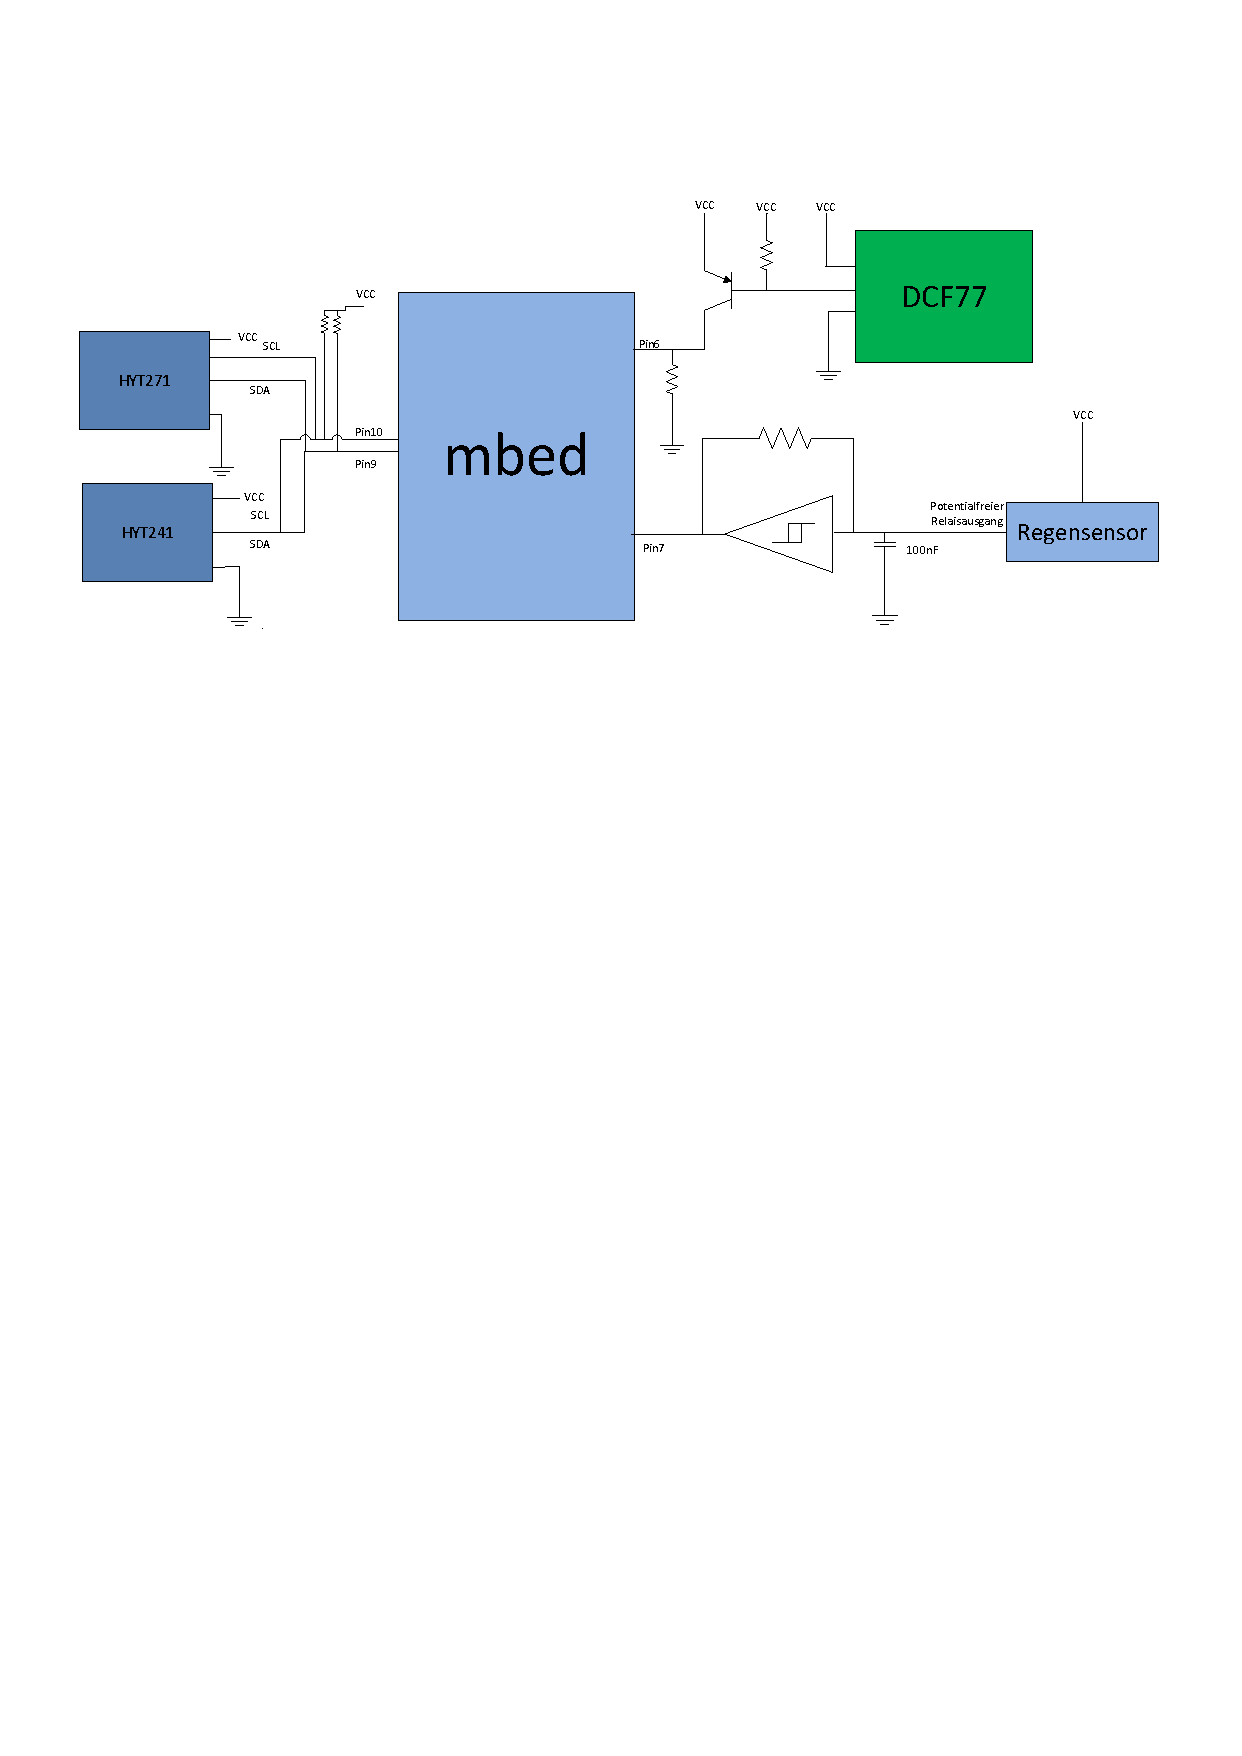
\includegraphics[width=\textwidth]{./Schaltplaene/Gesamt-Schaltung}
\caption{Gesamtschaltung des Projektes}
\label{fig:Gesamt-Schaltung}
\end{figure}
\subsubsection{Funktionsübersicht des Projektes}
\underline{\textbf{DCF77}}
\begin{description}
\item[timeDCF77* getTime()] Gibt die aktuell empfangene Zeit zurück.
\item[bool recieveTime()] Startet den Empfangsvorgang des DCF77 Empfängers.
\item[void setRTCClock()] Setzt die Real-Time-Clock des mbed Mikrocontrollers.
\item[void changeDebugState()] Lässt LEDs blinken wenn das DCF77 Signal empfangen wird. bzw. schaltet es wieder aus.
\end{description}
\underline{\textbf{HYT2x1}}
\begin{description}
\item[float getTemp()] Gibt die Aktuell empfangene Temperatur zurück.
\item[float getHumid()] Gibt die Aktuell empfangene relative Luftfeuchtigkeit zurück.
\item[bool update()] Startet einen neuen Messvorgang.
\item[bool setAdress()] Startet die Routine zum ändern der Adresse des HYT2x1. 
\end{description}
\underline{\textbf{Regensensor}}
\begin{description}
\item[getRain()] Gibt des aktuellen Regenstatus zurück.
\end{description}
\underline{\textbf{Logging}}
\begin{description}
\item[bool log(char Log[])] Schreibt den Parameter in den RAM des mbed Mikrocontrollers.
\end{description}

\subsubsection{DCF77 Empfangstabelle}
	\begin{table}[H]
		\begin{tabular}{ |l|p{7cm}| p{5cm}| }
			\hline \textbf{Bit} & \textbf{Bedeutung} & \textbf{Anmerkung} \\ 
			\hline 0 & Start einer neuen Minute & Ist immer 0 \\ 
			\hline 1-14 & Wetterinformationen der Firma MeteoTime und Katastrophenschutzinformationen & \\
			\hline 15 & Rufbit & \\
			\hline 16 & MEZ/MESZ Umstellung & 1: Am Ende dieser Stunde wird MEZ/MESZ umgestellt \\
			\hline 17 & MEZ Information & 0: MEZ, 1: MESZ \\
			\hline 18 & MEZ Information & 0: MESZ, 1: MEZ \\
			\hline 19 & Schaltsekunde & 1: Am Ende dieser Stunde wird eine Schaltsekunde eingefügt \\
			\hline 20 & Beginn der Zeitinformationen & Ist immer 1 \\
			\hline 21-27 & Minuten & \\
			\hline 28 & Parität Minuten & \\
			\hline 29-34 & Stunden & \\
			\hline 28 & Parität Stunden & \\
			\hline 36-41 & Kalendertag & \\
			\hline 42-44 & Wochentag & \\
			\hline 45-49 & Montsnummer & \\
			\hline 50-57 & Jahr & \\
			\hline 58 & Parität Datum & \\
			\hline 
		\end{tabular}
		\caption[DCF77 - Frameaufbau]{DCF77 - Frameaufbau, Quelle: \cite{DCF77Wiki}}
		\label{table:DCF77Frame}
	\end{table}



\end{document}